% chapter_12_L1T.tex -- chapter 12 of the JitJet book: the Level-1 trigger, the first checkpoint (Rule G of the
% Constitution: B1, B2, one section per step, B4, B5). ONE sample: the event with its pileup (Rule H: the signal and
% the pileup are followed apart only up to chapter 11).
% Every number comes from test/12_L1T/out/ (ledger_12_L1T.txt, l1t_12_L1T.log, settings_12_L1T.txt,
% truth_12_L1T.txt, the PNG pages); the companion doc/chapter/chapter_12_L1T.md lists them.

\chapter{12 -- L1T: the Level-1 trigger looks at the event and decides to keep it}
\label{ch:12_L1T}

\section{What this chapter is about}

Up to chapter~\ref{ch:11_DIGI} every stage did something \emph{to} the event: it added energy, removed energy or
changed its form. This stage does nothing to it. The Level-1 trigger (L1T) is the first of the two \emph{checkpoints}
of the journey: custom electronics that looks at every bunch crossing, 40 million times per second, and has about
four microseconds to say whether the crossing is worth reading out. It can keep about one crossing in four hundred
(some 100\,kHz); the High Level Trigger of chapter 13 then keeps a per cent or so of those. An event that the L1T
drops is gone: no later stage can recover it. In the simulation nothing is dropped, the decision is only recorded,
and the journey continues carrying the answer.

To be that fast the L1T does not use the digis of chapter~\ref{ch:11_DIGI}. It uses coarse copies made for it by
the detector front-ends, the \emph{trigger primitives}, from the calorimeters and the muon chambers only (the
tracker is too slow to read out at 40\,MHz in Run~3), and it processes them in six steps
(figure~\ref{fig:12_chain}), each a set of boards and, in CMSSW, a module of the sequence \code{SimL1Emulator}
(\path{L1Trigger/Configuration/python/SimL1Emulator_cff.py}), the bit-level emulation of the firmware that
\code{cmsDriver.py -s L1} runs:

\begin{enumerate}
\item \textbf{calorimeter trigger primitives}: one transverse energy per trigger tower from the ECAL and one from
the HCAL;
\item \textbf{calorimeter Layer-1} receives the primitives, calibrates them and sums ECAL and HCAL into trigger
towers;
\item \textbf{calorimeter Layer-2} builds from the towers the physics objects: jets, e/$\gamma$, $\tau$ and the
energy sums;
\item \textbf{muon trigger primitives and track finders}: the chambers send track stubs, three track finders (BMTF
in the barrel, OMTF in the overlap, EMTF in the endcaps) link them into muon candidates with a \pt;
\item \textbf{the global muon trigger} ($\mu$GMT, ``micro-GMT'') sorts the candidates, removes the duplicates and
keeps the best eight;
\item \textbf{the global trigger} ($\mu$GT) receives the calorimeter objects and the muons and evaluates every
algorithm of the \emph{menu} on them, all in parallel; if at least one fires, the event is kept.
\end{enumerate}

\begin{figure}[!htb]
\centering
\begin{tikzpicture}[x=0.93cm, font=\footnotesize, >={Stealth[length=2mm]},
  box/.style={draw, rounded corners=2pt, minimum height=10mm, text width=3.25cm, align=center, inner sep=2.5pt},
  calo/.style={box, fill=green!12}, mu/.style={box, fill=blue!10}, gt/.style={box, fill=red!12, text width=2.6cm, minimum height=22mm}]
\node[calo] (etp) at (0,1.75) {ECAL primitives\\{\tiny\ttfamily simEcalTriggerPrimitiveDigis}};
\node[calo] (htp) at (0,0.55) {HCAL primitives\\{\tiny\ttfamily simHcalTriggerPrimitiveDigis}};
\node[calo] (l1) at (4.25,1.15) {Layer-1: towers\\{\tiny\ttfamily simCaloStage2Layer1Digis}};
\node[calo] (l2) at (8.5,1.15) {Layer-2: jets, e/$\gamma$, $\tau$, sums\\{\tiny\ttfamily simCaloStage2Digis}};
\node[mu] (mtp) at (0,-1.45) {DT, CSC, RPC, GEM primitives\\{\tiny\ttfamily simDtTriggerPrimitiveDigis\\simCscTriggerPrimitiveDigis}};
\node[mu] (tf) at (4.25,-1.45) {BMTF, OMTF, EMTF\\{\tiny\ttfamily simKBmtf/simOmtf/simEmtfDigis}};
\node[mu] (gmt) at (8.5,-1.45) {$\mu$GMT: 8 muons\\{\tiny\ttfamily simGmtStage2Digis}};
\node[gt] (ugt) at (12.5,-0.15) {$\mu$GT: the menu\\{\tiny\ttfamily simGtStage2Digis}\\[3pt]$\rightarrow$ FinalOR};
\draw[->] (etp.east) -- (l1.west); \draw[->] (htp.east) -- (l1.west);
\draw[->] (l1) -- (l2); \draw[->] (l2.east) -- (ugt.west|-l2.east);
\draw[->] (mtp) -- (tf); \draw[->] (tf) -- (gmt); \draw[->] (gmt.east) -- (ugt.west|-gmt.east);
\node[font=\scriptsize, text=black!60] at (0,2.55) {step 1 (made in the DIGI job)};
\node[font=\scriptsize, text=black!60] at (4.25,1.95) {step 2};
\node[font=\scriptsize, text=black!60] at (8.5,1.95) {step 3};
\node[font=\scriptsize, text=black!60] at (2.1,-2.3) {step 4};
\node[font=\scriptsize, text=black!60] at (8.5,-2.3) {step 5};
\node[font=\scriptsize, text=black!60] at (12.5,1.25) {step 6};
\end{tikzpicture}
\caption{The Level-1 trigger of Run~3 (the ``stage-2'' trigger, in place since 2016) and the modules of the
\code{SimL1Emulator} sequence that emulate it. Calorimeter chain in green, muon chain in blue.}
\label{fig:12_chain}
\end{figure}

\begin{table}[!htb]
\centering\small\setlength{\tabcolsep}{4pt}
\caption{The six steps at a glance: what each one sends to the next, and how much of it there is in our event.
Every arrow of figure~\ref{fig:12_chain} is a reduction.}
\label{tab:12_glance}
\begin{tabular}{@{}c>{\raggedright\arraybackslash}p{3.2cm}>{\raggedright\arraybackslash}p{6.9cm}>{\raggedright\arraybackslash}p{4.3cm}@{}}
\toprule
step & who & sends, every 25\,ns & in our event \\
\midrule
1 & calorimeter front-ends & 8856 primitives: an 8-bit $E_{\mathrm T}$ and a few flag bits per tower & 2479 above zero, $2793\GeV$ \\
2 & Layer-1 & 5760 tower words of 16 bits: 9-bit $E_{\mathrm T}$, E/H ratio, flags & 2561 above zero, $2181\GeV$ \\
3 & Layer-2 & at most 12 jets, 12 e/$\gamma$, 12 $\tau$, and the energy sums & 9, 12, 12 \\
4 & muon chambers, track finders & stubs; then at most 3 candidates from each of 36 processors & 8 CSC stubs, 2 candidates \\
5 & $\mu$GMT & at most 8 muons & 1 \\
6 & $\mu$GT & 512 algorithm bits and their OR & 63 bits set, FinalOR 1 \\
\bottomrule
\end{tabular}
\end{table}

The chapter has one section per step. Each says what the step receives, what it does, with which parameters, what
the numbers of our event are, and shows the event in $\eta$--$\phi$ as it looks after the step. \emph{One} event is
followed (\path{test/12_L1T/run_12_L1T.sh}): the event as CMS sees it, the signal with the 71, 68 and 54 collisions
of bunch crossings $-1$, 0 and $+1$ on top. Chapter~\ref{ch:11_DIGI} was the last stage at which the signal and
the pileup existed apart; a trigger, like a detector, is only ever given their sum. Where the chapter needs to know
who made an object, it asks the truth that the file still carries: the two generator jets of
chapter~\ref{ch:07_GenJet}, and the simulated particles behind a muon.

\section{From the previous chapter}

One file of chapter~\ref{ch:11_DIGI} enters (Rule E), \path{test/11_DIGI/out/step3_DIGI_mixed_11_DIGI.root}: the
$544\,407$ digis of the signal with its pileup. The L1T uses very little of them. Of the $514\,881$ tracker digis it
uses none. Of the calorimeters it does not read the zero-suppressed data frames at all, but the two collections
that the \code{DIGI} job made from the unsuppressed frames for exactly this purpose,
\code{simEcalTriggerPrimitiveDigis} and \code{simHcalTriggerPrimitiveDigis}: section~\ref{sec:11_tp} of
chapter~\ref{ch:11_DIGI} explained what they are, how they are made and why they are made there. Step~1 of this
chapter was therefore computed in the previous job, and this is why \code{-s L1} cannot run on its own without two
extra lines (the companion, section~1). Of the muon system it uses the wire, strip and pad digis, 2016 of them.

What that section established, in four lines. The trigger sees the calorimeters on a grid of trigger towers,
$i\eta=\pm1\ldots\pm41$ and $i\phi=1\ldots72$ ($|i\eta|\leq17$ barrel, 18 to 28 endcap, 30 to 41 HF, 29 unused),
one 8-bit transverse energy per tower and bunch crossing, $0.5\GeV$ per count. A primitive measures the energy
deposited in its tower to half a GeV, but a tower with less than that sends nothing, and noise alone makes one
tower in nine send a count. Of the $2793\GeV$ of primitives of our event, the signal alone would have sent
$536.5\GeV$, more than half of it noise: four fifths of what the trigger receives is pileup and noise.\footnote{All numbers of this chapter are in
\path{test/12_L1T/out/}: \path{ledger_12_L1T.txt} (step by step), \path{l1t_12_L1T.log} (the analyzers
\code{L1TCaloAnalyzer}, \code{L1TMuonAnalyzer}, \code{L1TGlobalAnalyzer}), \path{settings_12_L1T.txt} (the module
parameters) and \path{truth_12_L1T.txt}; the companion lists them. Numbers about the signal alone are quoted from
chapter~\ref{ch:11_DIGI}.}

The job runs with the 2025 settings of the release: the menu of the global tag is
\path{L1Menu_Collisions2025_v1_0_0}, the ECAL primitives of chapter~\ref{ch:11_DIGI} were made with the payloads of 2025, and the era \code{Run3\_2025}
brings the CICADA model of 2025; the calorimeter-trigger parameters of Layer-1 and Layer-2 and the muon payloads are
those of 2024. The first version of this chapter ran with the 2024 settings; what the
change did to the decision is told in the ledger section.

What is kept: everything. The \code{L1} process copies its input and adds its products under the process name
\code{L1}, about fifty collections, the output of every board of figure~\ref{fig:12_chain}. What changes is the
granularity at which the event is looked at: half a million digis become, for the trigger, 8856 small integers.

\section{Step 1: the calorimeter trigger primitives}

\textbf{What the step does.} Every 25\,ns each calorimeter front-end sends one transverse energy per trigger tower
to Layer-1 on optical links: 4032 from the ECAL, 4032 from HB and HE, 792 from the HF. The primitive of a tower is
a small time series (five consecutive crossings for the ECAL, four for the HCAL), and the trigger takes one value
per crossing: for our event the one of bunch crossing 0, the \emph{sample of interest}. The emulator of the
calorimeter trigger processes this crossing only (\path{L1Trigger/L1TCaloLayer1/plugins/L1TCaloLayer1.cc}: ``Currently
we only read and process the `hit' BX only''); in the detector the crossings $-1$ and $+1$, with their 71 and 54
collisions, go through the same six steps as events of their own.

\textbf{The numbers of the event.} Table~\ref{tab:12_tp} counts what arrives, and figure~\ref{fig:12_tp} shows it.

\begin{table}[!htb]
\centering\small
\caption{Step 1: the trigger primitives of bunch crossing 0 (\code{ledger\_12\_L1T.txt}, section 1).}
\label{tab:12_tp}
\begin{tabular}{l rrrr}
\toprule
 & primitives & with $E_{\mathrm T}>0$ & $\sum E_{\mathrm T}$ [GeV] & largest [GeV] \\
\midrule
ECAL barrel (EB), $|i\eta|\leq17$ & 2448 & 683 & 468.0 & 5.5 \\
ECAL endcap (EE), $18\leq|i\eta|\leq28$ & 1584 & 494 & 579.5 & 7.0 \\
HCAL barrel (HB), $|i\eta|\leq16$ & 2304 & 233 & 183.0 & 7.5 \\
HCAL endcap (HE), $17\leq|i\eta|\leq28$ & 1728 & 328 & 241.5 & 10.0 \\
HF, $30\leq|i\eta|\leq41$ & 792 & 741 & 1321.0 & 90.5 \\
\midrule
all & 8856 & 2479 & 2793.0 & 90.5 \\
\bottomrule
\end{tabular}
\end{table}

\emph{Where the energy is.} Two thirds of it are in two places: the HF ($1321\GeV$, 741 of its 792 primitives
are lit) and the endcap ECAL ($579.5\GeV$). The barrel, with more than half of the towers, holds $651\GeV$. The
pileup is roughly flat in $\eta$, the towers are not: a tower at the edge of the endcap is four times larger than
a barrel tower and collects several soft particles where a barrel tower collects a fraction of one, so that the
half-GeV count that hides most of the pileup in the barrel does not hide it there. In figure~\ref{fig:12_tp} the
rings at $2.5<\abseta<3$ of the ECAL and the whole HF are bands of one to a few GeV per tower, and the barrel a dust
of one- and two-count towers, many of them noise.

\emph{The two jets look completely different.} The $\bar b$ jet ($\pt=115.9\GeV$ at $\eta=-3.75$) falls in the
HF, where a jet is narrow in tower units: one primitive at $i\eta=-34$ carries $90.5\GeV$ and its neighbour at
$i\eta=-33$ another $15.5\GeV$; the $9\times9$ towers around it hold $199.75\GeV$. The $b$ jet sits on the
barrel--endcap boundary, $\eta=-1.59$, and is spread over a dozen towers (figure~\ref{fig:12_tpzoom}): a column of
ECAL towers at $i\eta=-19$ with $7.0$, $6.0$ and $5.0\GeV$ and three HCAL towers with $10.0$, $4.5$ and
$3.5\GeV$; no tower of either calorimeter is above $10\GeV$. Its generator jet has $117.8\GeV$, of which
$37.5\GeV$ are the neutrino of the semileptonic $B^-$ decay of chapter~\ref{ch:06_Decay}; what a calorimeter can
see at best is the $79.8\GeV$ of chapter~\ref{ch:07_GenJet}. In the $9\times9$ towers around it the ECAL
primitives add up to $46.0\GeV$ and the HCAL ones to $28.0\GeV$, pileup included. The jet that the trigger will
build is still visible in figure~\ref{fig:12_tp} only because it is in a quiet region of the detector.

\begin{figure}[!htb]
\centering
\includegraphics[width=0.47\textwidth,trim=0 0 475 0,clip]{12_L1T/out/l1t_12_L1T_calo_ecaltp_run1_event1.png}\hfill
\includegraphics[width=0.47\textwidth,trim=0 0 475 0,clip]{12_L1T/out/l1t_12_L1T_calo_hcaltp_run1_event1.png}
\caption{Step 1, the trigger primitives of the event on the trigger-tower grid, one coloured cell per tower, colour
= $E_{\mathrm T}$ on a logarithmic scale from $0.25$ to $256\GeV$
(\code{l1t\_12\_L1T\_calo\_ecaltp/hcaltp\_run1\_event1.png}). Left: ECAL; right: HCAL, with the HF beyond
$\abseta=3$. Magenta circles: the two \code{ak4GenJets} of chapter~\ref{ch:07_GenJet}. The dotted lines are the
barrel--endcap and endcap--HF boundaries.}
\label{fig:12_tp}
\end{figure}

\begin{figure}[!htb]
\centering
\includegraphics[width=0.47\textwidth,trim=0 0 475 0,clip]{12_L1T/out/l1t_12_L1T_calo_jet2_ecaltp_run1_event1.png}\hfill
\includegraphics[width=0.47\textwidth,trim=0 0 475 0,clip]{12_L1T/out/l1t_12_L1T_calo_jet2_hcaltp_run1_event1.png}
\caption{Step 1, the $b$ jet tower by tower: the ECAL primitives (left) and the HCAL primitives (right) of the
$17\times17$ towers around $(i\eta,i\phi)=(-18,50)$, one square per tower with its $E_{\mathrm T}$ in GeV
(\code{l1t\_12\_L1T\_calo\_jet2\_ecaltp/hcaltp\_run1\_event1.png}). The red square is the $9\times9$ window that step~3
will use; it holds $46.0\GeV$ of ECAL and $28.0\GeV$ of HCAL primitives. The towers outside the jet are the pileup
and the noise.}
\label{fig:12_tpzoom}
\end{figure}

\section{Step 2: calorimeter Layer-1}

\textbf{What the step does.} Layer-1 (18 processing cards in the hardware, the classes \code{UCTLayer1},
\code{UCTCard}, \code{UCTRegion}, \code{UCTTower} of \path{L1Trigger/L1TCaloLayer1} in the emulator) does three
things to every tower. It \emph{receives} the two primitives of the tower and aligns them in time. It
\emph{calibrates} each with a lookup table addressed by the 8-bit value and the tower ring: the table multiplies
the transverse energy by a scale factor that depends on $|i\eta|$ and on the energy, in 14 energy bins from below
$3\GeV$ to above $70\GeV$. And it \emph{sums} the calibrated ECAL and HCAL values into one tower word of 16 bits:
9 bits of $E_{\mathrm T}$ ($0.5\GeV$ per count, saturating at $255.5\GeV$), 3 bits for the ratio of the two
energies on a logarithmic scale, and flag bits (which of the two is larger, the ECAL fine-grain bit, an HCAL
feature bit). The towers of a ring are then sorted and sent to Layer-2. It is the first place where the ECAL and
the HCAL energy of the same $\eta$--$\phi$ cell meet. The scale factors are not in the configuration: they are the
payload \code{L1TCaloParams\_static\_2024\_v0\_1\_mc} of the record \code{L1TCaloParamsRcd} in the global tag, the same
numbers as \path{L1Trigger/L1TCalorimeter/python/caloParams_2024_v0_1_cfi.py}; the analyzer prints the three tables
(companion, section~4).

\textbf{The parameters.} Table~\ref{tab:12_sf} is what the tables do. For the ECAL the factor is a calibration,
$1.12$ at low energy falling to $1.01$ at high energy, with one exception: it is \emph{zero} for the three last
rings of the endcap below a threshold ($3\GeV$ for ring 26, $6\GeV$ for 27, $9\GeV$ for 28). For the HCAL it is 1
everywhere, except that one-count primitives ($0.5\GeV$) are set to zero for $|i\eta|\leq15$ (the comment in the
python file reads ``ZERO-SUPPRESS $<$1GeV (i.e. 0.5GeV) IN THE BARREL ONLY''). For the HF it is 1, but the
primitive is divided between the two (or four) $5^\circ$ towers it covers, each getting half (a quarter) of it
\emph{rounded down} to half a GeV (\path{L1Trigger/L1TCaloLayer1/src/L1TCaloLayer1FetchLUTs.cc}: ``Divide by two
(since two duplicate towers are sent)''), so that a one-count HF primitive disappears. Three zero suppressions,
then, hidden in what is called a calibration, each aimed at the pileup and the noise of step~1.

\begin{table}[!htb]
\centering\small\setlength{\tabcolsep}{4.5pt}
\caption{Step 2: the Layer-1 scale factors of the global tag (\code{l1t\_12\_L1T.log}, lines
\code{caloParams layer1...ScaleFactors}), for some rings and three of the 14 bins of the primitive's $E_{\mathrm T}$.}
\label{tab:12_sf}
\begin{tabular}{l ccccccc}
\toprule
ring $|i\eta|$ & 1 & 15 & 17 & 18 & 25 & 26 / 27 / 28 & 30--41 (HF) \\
\midrule
ECAL, $E_{\mathrm T}<3\GeV$ & 1.12 & 1.13 & 1.14 & 1.26 & 1.19 & 0 / 0 / 0 & \\
ECAL, $6<E_{\mathrm T}<9\GeV$ & 1.08 & 1.10 & 1.10 & 1.23 & 1.15 & 1.14 / 1.14 / 0 & \\
ECAL, $E_{\mathrm T}>70\GeV$ & 1.02 & 1.02 & 1.02 & 1.04 & 1.02 & 1.02 / 1.00 / 1.01 & \\
HCAL, $E_{\mathrm T}<1\GeV$ & 0 & 0 & 1 & 1 & 1 & 1 / 1 / 1 & 1, then $\div2$ ($\div4$) \\
HCAL, $E_{\mathrm T}\geq1\GeV$ & 1 & 1 & 1 & 1 & 1 & 1 / 1 / 1 & 1, then $\div2$ ($\div4$) \\
\bottomrule
\end{tabular}
\end{table}

\textbf{The numbers of the event.} The step removes a fifth of what it receives (table~\ref{tab:12_l1}): $307\GeV$
of the $1047.5\GeV$ of ECAL primitives and $226\GeV$ of the $1321\GeV$ of the HF. Figure~\ref{fig:12_rings} shows
where, ring by ring. The ECAL loss is all in the last three rings of the endcap: rings 26 to 28 receive
$445.5\GeV$, $321.5\GeV$ of it from the ECAL, and come out with $134.5\GeV$. In rings 27 and 28 not one ECAL
primitive reaches the 6 and $9\GeV$ of table~\ref{tab:12_sf}, and only the HCAL is left (the ring $i\eta=+28$
receives $68\GeV$ of ECAL and $36\GeV$ of HCAL primitives and keeps $36\GeV$). The HF loses a little in every ring,
to the rounding. The barrel and the rest of the endcap are hardly touched: the barrel rings receive $655\GeV$ and
keep $576.5\GeV$. After the step the event is 2561 towers and $2181\GeV$, and the bright bands of
figure~\ref{fig:12_l1} are the HF. With the 2024 conditions they were not alone: the ECAL primitives of ring~28 were
four times larger ($315\GeV$ in ring $+28$, up to $11.5\GeV$ each), many survived the $9\GeV$ cut, the ring kept
$181\GeV$, and step~3 seeded six pileup jets in it. The crystals of ring~28 have lost transparency: the 2025
digitiser scales their light by 0.025 instead of 0.096 (chapter~\ref{ch:11_DIGI}), and the larger linearisation
constants of the 2025 primitives ($\times1.37$ there) give back only part of it: per GeV deposited, a ring-28
primitive is 0.36 of what it was in 2024 (0.94 to 0.99 up to ring 23; companion, last section).

\begin{table}[!htb]
\centering\small
\caption{Step 2: what Layer-1 makes of the primitives, summed transverse energy in GeV in and out of the step
(\code{ledger\_12\_L1T.txt}, sections 1 and 2).}
\label{tab:12_l1}
\begin{tabular}{l rrr c l rr}
\toprule
 & in & out & change & & towers after the step & $E_{\mathrm T}>0$ & $\sum E_{\mathrm T}$ \\
\cmidrule(lr){1-4}\cmidrule(lr){6-8}
ECAL (EB + EE) & 1047.5 & 740.5 & $-307.0$ & & barrel, $|i\eta|\leq17$ & 738 & 576.5 \\
HCAL (HB + HE) & 424.5 & 345.5 & $-79.0$ & & endcap, $18\leq|i\eta|\leq28$ & 557 & 509.5 \\
HF & 1321.0 & 1095.0 & $-226.0$ & & forward, $|i\eta|\geq30$ & 1266 & 1095.0 \\
all & 2793.0 & 2181.0 & $-612.0$ & & all (of 5760) & 2561 & 2181.0 \\
\bottomrule
\end{tabular}
\end{table}

\begin{figure}[!htb]
\centering
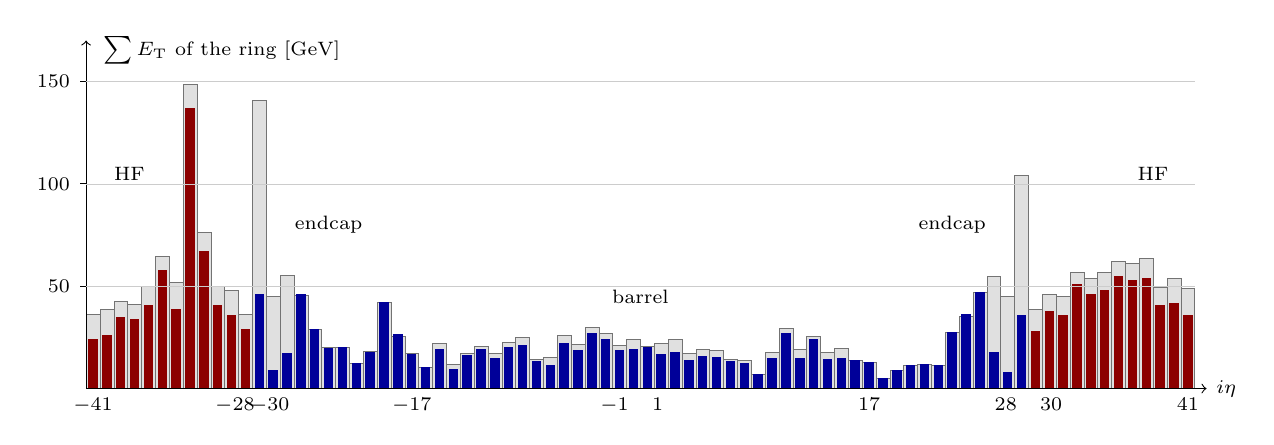
\begin{tikzpicture}[x=1cm, y=0.026cm, font=\scriptsize]
\draw[black!55, fill=black!12, line width=0.2pt] (0.000,0) rectangle (0.176,36.5);
\fill[red!55!black] (0.028,0) rectangle (0.148,24.0);
\draw[black!55, fill=black!12, line width=0.2pt] (0.176,0) rectangle (0.352,38.5);
\fill[red!55!black] (0.204,0) rectangle (0.324,26.0);
\draw[black!55, fill=black!12, line width=0.2pt] (0.352,0) rectangle (0.528,42.5);
\fill[red!55!black] (0.380,0) rectangle (0.500,35.0);
\draw[black!55, fill=black!12, line width=0.2pt] (0.528,0) rectangle (0.704,41.0);
\fill[red!55!black] (0.556,0) rectangle (0.676,34.0);
\draw[black!55, fill=black!12, line width=0.2pt] (0.704,0) rectangle (0.880,50.0);
\fill[red!55!black] (0.732,0) rectangle (0.852,41.0);
\draw[black!55, fill=black!12, line width=0.2pt] (0.880,0) rectangle (1.056,64.5);
\fill[red!55!black] (0.908,0) rectangle (1.028,58.0);
\draw[black!55, fill=black!12, line width=0.2pt] (1.056,0) rectangle (1.232,52.0);
\fill[red!55!black] (1.084,0) rectangle (1.204,39.0);
\draw[black!55, fill=black!12, line width=0.2pt] (1.232,0) rectangle (1.408,148.5);
\fill[red!55!black] (1.260,0) rectangle (1.380,137.0);
\draw[black!55, fill=black!12, line width=0.2pt] (1.408,0) rectangle (1.584,76.5);
\fill[red!55!black] (1.436,0) rectangle (1.556,67.0);
\draw[black!55, fill=black!12, line width=0.2pt] (1.584,0) rectangle (1.760,50.0);
\fill[red!55!black] (1.612,0) rectangle (1.732,41.0);
\draw[black!55, fill=black!12, line width=0.2pt] (1.760,0) rectangle (1.936,48.0);
\fill[red!55!black] (1.788,0) rectangle (1.908,36.0);
\draw[black!55, fill=black!12, line width=0.2pt] (1.936,0) rectangle (2.112,36.5);
\fill[red!55!black] (1.964,0) rectangle (2.084,29.0);
\draw[black!55, fill=black!12, line width=0.2pt] (2.112,0) rectangle (2.288,141.0);
\fill[blue!60!black] (2.140,0) rectangle (2.260,46.0);
\draw[black!55, fill=black!12, line width=0.2pt] (2.288,0) rectangle (2.464,45.0);
\fill[blue!60!black] (2.316,0) rectangle (2.436,9.0);
\draw[black!55, fill=black!12, line width=0.2pt] (2.464,0) rectangle (2.640,55.5);
\fill[blue!60!black] (2.492,0) rectangle (2.612,17.5);
\draw[black!55, fill=black!12, line width=0.2pt] (2.640,0) rectangle (2.816,45.5);
\fill[blue!60!black] (2.668,0) rectangle (2.788,46.0);
\draw[black!55, fill=black!12, line width=0.2pt] (2.816,0) rectangle (2.992,29.0);
\fill[blue!60!black] (2.844,0) rectangle (2.964,29.0);
\draw[black!55, fill=black!12, line width=0.2pt] (2.992,0) rectangle (3.168,20.0);
\fill[blue!60!black] (3.020,0) rectangle (3.140,20.0);
\draw[black!55, fill=black!12, line width=0.2pt] (3.168,0) rectangle (3.344,20.0);
\fill[blue!60!black] (3.196,0) rectangle (3.316,20.5);
\draw[black!55, fill=black!12, line width=0.2pt] (3.344,0) rectangle (3.520,12.5);
\fill[blue!60!black] (3.372,0) rectangle (3.492,12.5);
\draw[black!55, fill=black!12, line width=0.2pt] (3.520,0) rectangle (3.696,18.0);
\fill[blue!60!black] (3.548,0) rectangle (3.668,18.0);
\draw[black!55, fill=black!12, line width=0.2pt] (3.696,0) rectangle (3.872,42.0);
\fill[blue!60!black] (3.724,0) rectangle (3.844,42.5);
\draw[black!55, fill=black!12, line width=0.2pt] (3.872,0) rectangle (4.048,25.5);
\fill[blue!60!black] (3.900,0) rectangle (4.020,26.5);
\draw[black!55, fill=black!12, line width=0.2pt] (4.048,0) rectangle (4.224,17.0);
\fill[blue!60!black] (4.076,0) rectangle (4.196,17.0);
\draw[black!55, fill=black!12, line width=0.2pt] (4.224,0) rectangle (4.400,10.5);
\fill[blue!60!black] (4.252,0) rectangle (4.372,10.5);
\draw[black!55, fill=black!12, line width=0.2pt] (4.400,0) rectangle (4.576,22.0);
\fill[blue!60!black] (4.428,0) rectangle (4.548,19.5);
\draw[black!55, fill=black!12, line width=0.2pt] (4.576,0) rectangle (4.752,12.0);
\fill[blue!60!black] (4.604,0) rectangle (4.724,9.5);
\draw[black!55, fill=black!12, line width=0.2pt] (4.752,0) rectangle (4.928,17.0);
\fill[blue!60!black] (4.780,0) rectangle (4.900,16.5);
\draw[black!55, fill=black!12, line width=0.2pt] (4.928,0) rectangle (5.104,20.5);
\fill[blue!60!black] (4.956,0) rectangle (5.076,19.5);
\draw[black!55, fill=black!12, line width=0.2pt] (5.104,0) rectangle (5.280,17.0);
\fill[blue!60!black] (5.132,0) rectangle (5.252,15.0);
\draw[black!55, fill=black!12, line width=0.2pt] (5.280,0) rectangle (5.456,22.5);
\fill[blue!60!black] (5.308,0) rectangle (5.428,20.5);
\draw[black!55, fill=black!12, line width=0.2pt] (5.456,0) rectangle (5.632,25.0);
\fill[blue!60!black] (5.484,0) rectangle (5.604,21.5);
\draw[black!55, fill=black!12, line width=0.2pt] (5.632,0) rectangle (5.808,14.5);
\fill[blue!60!black] (5.660,0) rectangle (5.780,13.5);
\draw[black!55, fill=black!12, line width=0.2pt] (5.808,0) rectangle (5.984,15.5);
\fill[blue!60!black] (5.836,0) rectangle (5.956,11.5);
\draw[black!55, fill=black!12, line width=0.2pt] (5.984,0) rectangle (6.160,26.0);
\fill[blue!60!black] (6.012,0) rectangle (6.132,22.0);
\draw[black!55, fill=black!12, line width=0.2pt] (6.160,0) rectangle (6.336,21.5);
\fill[blue!60!black] (6.188,0) rectangle (6.308,19.0);
\draw[black!55, fill=black!12, line width=0.2pt] (6.336,0) rectangle (6.512,30.0);
\fill[blue!60!black] (6.364,0) rectangle (6.484,27.0);
\draw[black!55, fill=black!12, line width=0.2pt] (6.512,0) rectangle (6.688,27.0);
\fill[blue!60!black] (6.540,0) rectangle (6.660,24.0);
\draw[black!55, fill=black!12, line width=0.2pt] (6.688,0) rectangle (6.864,21.0);
\fill[blue!60!black] (6.716,0) rectangle (6.836,19.0);
\draw[black!55, fill=black!12, line width=0.2pt] (6.864,0) rectangle (7.040,24.0);
\fill[blue!60!black] (6.892,0) rectangle (7.012,19.5);
\draw[black!55, fill=black!12, line width=0.2pt] (7.040,0) rectangle (7.216,20.5);
\fill[blue!60!black] (7.068,0) rectangle (7.188,20.5);
\draw[black!55, fill=black!12, line width=0.2pt] (7.216,0) rectangle (7.392,22.0);
\fill[blue!60!black] (7.244,0) rectangle (7.364,17.0);
\draw[black!55, fill=black!12, line width=0.2pt] (7.392,0) rectangle (7.568,24.0);
\fill[blue!60!black] (7.420,0) rectangle (7.540,18.0);
\draw[black!55, fill=black!12, line width=0.2pt] (7.568,0) rectangle (7.744,17.0);
\fill[blue!60!black] (7.596,0) rectangle (7.716,14.0);
\draw[black!55, fill=black!12, line width=0.2pt] (7.744,0) rectangle (7.920,19.0);
\fill[blue!60!black] (7.772,0) rectangle (7.892,16.0);
\draw[black!55, fill=black!12, line width=0.2pt] (7.920,0) rectangle (8.096,18.5);
\fill[blue!60!black] (7.948,0) rectangle (8.068,15.5);
\draw[black!55, fill=black!12, line width=0.2pt] (8.096,0) rectangle (8.272,14.5);
\fill[blue!60!black] (8.124,0) rectangle (8.244,13.5);
\draw[black!55, fill=black!12, line width=0.2pt] (8.272,0) rectangle (8.448,14.0);
\fill[blue!60!black] (8.300,0) rectangle (8.420,12.5);
\draw[black!55, fill=black!12, line width=0.2pt] (8.448,0) rectangle (8.624,7.0);
\fill[blue!60!black] (8.476,0) rectangle (8.596,7.0);
\draw[black!55, fill=black!12, line width=0.2pt] (8.624,0) rectangle (8.800,17.5);
\fill[blue!60!black] (8.652,0) rectangle (8.772,15.0);
\draw[black!55, fill=black!12, line width=0.2pt] (8.800,0) rectangle (8.976,29.5);
\fill[blue!60!black] (8.828,0) rectangle (8.948,27.0);
\draw[black!55, fill=black!12, line width=0.2pt] (8.976,0) rectangle (9.152,19.0);
\fill[blue!60!black] (9.004,0) rectangle (9.124,15.0);
\draw[black!55, fill=black!12, line width=0.2pt] (9.152,0) rectangle (9.328,25.5);
\fill[blue!60!black] (9.180,0) rectangle (9.300,24.0);
\draw[black!55, fill=black!12, line width=0.2pt] (9.328,0) rectangle (9.504,17.5);
\fill[blue!60!black] (9.356,0) rectangle (9.476,14.5);
\draw[black!55, fill=black!12, line width=0.2pt] (9.504,0) rectangle (9.680,19.5);
\fill[blue!60!black] (9.532,0) rectangle (9.652,15.0);
\draw[black!55, fill=black!12, line width=0.2pt] (9.680,0) rectangle (9.856,14.0);
\fill[blue!60!black] (9.708,0) rectangle (9.828,14.0);
\draw[black!55, fill=black!12, line width=0.2pt] (9.856,0) rectangle (10.032,13.0);
\fill[blue!60!black] (9.884,0) rectangle (10.004,13.0);
\draw[black!55, fill=black!12, line width=0.2pt] (10.032,0) rectangle (10.208,5.0);
\fill[blue!60!black] (10.060,0) rectangle (10.180,5.0);
\draw[black!55, fill=black!12, line width=0.2pt] (10.208,0) rectangle (10.384,9.0);
\fill[blue!60!black] (10.236,0) rectangle (10.356,9.0);
\draw[black!55, fill=black!12, line width=0.2pt] (10.384,0) rectangle (10.560,11.5);
\fill[blue!60!black] (10.412,0) rectangle (10.532,11.5);
\draw[black!55, fill=black!12, line width=0.2pt] (10.560,0) rectangle (10.736,12.0);
\fill[blue!60!black] (10.588,0) rectangle (10.708,12.0);
\draw[black!55, fill=black!12, line width=0.2pt] (10.736,0) rectangle (10.912,11.5);
\fill[blue!60!black] (10.764,0) rectangle (10.884,11.5);
\draw[black!55, fill=black!12, line width=0.2pt] (10.912,0) rectangle (11.088,27.5);
\fill[blue!60!black] (10.940,0) rectangle (11.060,27.5);
\draw[black!55, fill=black!12, line width=0.2pt] (11.088,0) rectangle (11.264,35.5);
\fill[blue!60!black] (11.116,0) rectangle (11.236,36.5);
\draw[black!55, fill=black!12, line width=0.2pt] (11.264,0) rectangle (11.440,47.0);
\fill[blue!60!black] (11.292,0) rectangle (11.412,47.0);
\draw[black!55, fill=black!12, line width=0.2pt] (11.440,0) rectangle (11.616,55.0);
\fill[blue!60!black] (11.468,0) rectangle (11.588,18.0);
\draw[black!55, fill=black!12, line width=0.2pt] (11.616,0) rectangle (11.792,45.0);
\fill[blue!60!black] (11.644,0) rectangle (11.764,8.0);
\draw[black!55, fill=black!12, line width=0.2pt] (11.792,0) rectangle (11.968,104.0);
\fill[blue!60!black] (11.820,0) rectangle (11.940,36.0);
\draw[black!55, fill=black!12, line width=0.2pt] (11.968,0) rectangle (12.144,38.5);
\fill[red!55!black] (11.996,0) rectangle (12.116,28.0);
\draw[black!55, fill=black!12, line width=0.2pt] (12.144,0) rectangle (12.320,46.0);
\fill[red!55!black] (12.172,0) rectangle (12.292,38.0);
\draw[black!55, fill=black!12, line width=0.2pt] (12.320,0) rectangle (12.496,45.0);
\fill[red!55!black] (12.348,0) rectangle (12.468,36.0);
\draw[black!55, fill=black!12, line width=0.2pt] (12.496,0) rectangle (12.672,57.0);
\fill[red!55!black] (12.524,0) rectangle (12.644,51.0);
\draw[black!55, fill=black!12, line width=0.2pt] (12.672,0) rectangle (12.848,54.0);
\fill[red!55!black] (12.700,0) rectangle (12.820,46.0);
\draw[black!55, fill=black!12, line width=0.2pt] (12.848,0) rectangle (13.024,57.0);
\fill[red!55!black] (12.876,0) rectangle (12.996,48.0);
\draw[black!55, fill=black!12, line width=0.2pt] (13.024,0) rectangle (13.200,62.0);
\fill[red!55!black] (13.052,0) rectangle (13.172,55.0);
\draw[black!55, fill=black!12, line width=0.2pt] (13.200,0) rectangle (13.376,61.0);
\fill[red!55!black] (13.228,0) rectangle (13.348,53.0);
\draw[black!55, fill=black!12, line width=0.2pt] (13.376,0) rectangle (13.552,63.5);
\fill[red!55!black] (13.404,0) rectangle (13.524,54.0);
\draw[black!55, fill=black!12, line width=0.2pt] (13.552,0) rectangle (13.728,49.5);
\fill[red!55!black] (13.580,0) rectangle (13.700,41.0);
\draw[black!55, fill=black!12, line width=0.2pt] (13.728,0) rectangle (13.904,54.0);
\fill[red!55!black] (13.756,0) rectangle (13.876,42.0);
\draw[black!55, fill=black!12, line width=0.2pt] (13.904,0) rectangle (14.080,49.0);
\fill[red!55!black] (13.932,0) rectangle (14.052,36.0);
\draw[->] (0,0) -- (14.23,0) node[right] {$i\eta$};
\draw[->] (0,0) -- (0,170);
\node[anchor=west] at (0.1,165) {$\sum E_{\mathrm T}$ of the ring [GeV]};
\draw (0,50) -- (-0.08,50) node[left] {50};
\draw[black!20, line width=0.2pt] (0,50) -- (14.08,50);
\draw (0,100) -- (-0.08,100) node[left] {100};
\draw[black!20, line width=0.2pt] (0,100) -- (14.08,100);
\draw (0,150) -- (-0.08,150) node[left] {150};
\draw[black!20, line width=0.2pt] (0,150) -- (14.08,150);
\node[anchor=north, inner sep=1.5pt] at (0.088,-2.5) {$-41$};
\node[anchor=north west, inner sep=1.5pt] at (2.024,-2.5) {$-30$};
\node[anchor=north east, inner sep=1.5pt] at (2.200,-2.5) {$-28$};
\node[anchor=north, inner sep=1.5pt] at (4.136,-2.5) {$-17$};
\node[anchor=north east, inner sep=1.5pt] at (6.952,-2.5) {$-1$};
\node[anchor=north west, inner sep=1.5pt] at (7.128,-2.5) {1};
\node[anchor=north, inner sep=1.5pt] at (9.944,-2.5) {17};
\node[anchor=north east, inner sep=1.5pt] at (11.880,-2.5) {28};
\node[anchor=north west, inner sep=1.5pt] at (12.056,-2.5) {30};
\node[anchor=north, inner sep=1.5pt] at (13.992,-2.5) {41};
\node at (0.55,105) {HF};
\node at (3.08,80) {endcap};
\node at (7.04,45) {barrel};
\node at (11.00,80) {endcap};
\node at (13.55,105) {HF};
\end{tikzpicture}
\caption{Step 2 ring by ring: the summed $E_{\mathrm T}$ of the 72 towers of each $\eta$ ring
(\code{ledger\_12\_L1T.txt}, section 2). Grey: the ECAL + HCAL primitives that enter Layer-1; colour: the towers that
leave it (blue: barrel and endcap, red: HF). The grey above the colour is what the step removes: the low primitives
of ECAL rings 26 to 28, and the rounding of the HF primitives. The two spikes in the HF at $i\eta=-34,-33$ are the
$\bar b$ jet.}
\label{fig:12_rings}
\end{figure}

Figure~\ref{fig:12_hfzoom} shows the step at work on the $\bar b$ jet: the $90.5\GeV$ primitive at $i\eta=-34$
becomes two towers of $45.0\GeV$ side by side in $\phi$, the $15.5\GeV$ one next to it two towers of $7.5\GeV$
(half a GeV is lost in the rounding each time), and every primitive of $0.5\GeV$ vanishes: $199.75\GeV$ of
primitives in the window, $189.0\GeV$ of towers. For the $b$ jet the seed tower $(-18,50)$ becomes
$3.5\times1.26\rightarrow4.0\GeV$ of ECAL plus $10.0\GeV$ of HCAL, a tower of $14.0\GeV$.

\begin{plainwords}[One tower word, bit by bit]
The tower $(-18,50)$ leaves Layer-1 as 16 bits (\path{L1Trigger/L1TCaloLayer1/src/UCTTower.cc}). Bits 0 to 8:
$E_{\mathrm T}=28$ counts, $14.0\GeV$, the sum of 8 counts of ECAL and 20 of HCAL. Bits 9 to 11: the ratio code 1,
the difference of the two energies in powers of two ($\log_2 20=4$, $\log_2 8=3$). Bit 12, ``one of the two is
zero'': 0. Bit 13, ``the ECAL is the larger'': 0, this tower is hadronic. Bits 14 and 15, the HCAL feature bit and
the ECAL fine-grain bit: 0. Layer-2 never sees the two energies separately: for its jets it uses the first nine
bits, for electrons and photons the ratio and the flags. The tower $(-4,4)$, with $6.0\GeV$ of ECAL and no HCAL,
has bits 12 and 13 set; the HF tower $(-34,11)$ of the $\bar b$ jet, $45.0\GeV$, has bit 12 (an HF tower has no
ECAL) and bit 14, which in the HF means ``above the minimum-bias threshold''.
\end{plainwords}

\begin{figure}[!htb]
\centering
\includegraphics[width=0.47\textwidth,trim=0 0 475 0,clip]{12_L1T/out/l1t_12_L1T_calo_jet1_hcaltp_run1_event1.png}\hfill
\includegraphics[width=0.47\textwidth,trim=0 0 475 0,clip]{12_L1T/out/l1t_12_L1T_calo_jet1_layer1_run1_event1.png}
\caption{Step 2 at work on the $\bar b$ jet, in the HF: the HCAL primitives (left; a primitive is two towers wide
in $\phi$, four for $|i\eta|\geq40$, the grey frames) and the Layer-1 towers made of them (right)
(\code{l1t\_12\_L1T\_calo\_jet1\_hcaltp/layer1\_run1\_event1.png}). Each primitive is shared between its towers and rounded
down to $0.5\GeV$; the black square is the seed tower of step~3, $(i\eta,i\phi)=(-34,12)$, the red one its
$9\times9$ window. The column at $i\eta=-28$, on the right, is the last ring of the endcap.}
\label{fig:12_hfzoom}
\end{figure}

\begin{figure}[!htb]
\centering
\includegraphics[width=0.93\textwidth]{12_L1T/out/l1t_12_L1T_calo_layer1_run1_event1.png}
\caption{Step 2, the Layer-1 towers of the event (ECAL + HCAL, calibrated): 2561 towers, $2181\GeV$
(\code{l1t\_12\_L1T\_calo\_layer1\_run1\_event1.png}). This map is the whole input of step 3.}
\label{fig:12_l1}
\end{figure}

\section{Step 3: calorimeter Layer-2}

\textbf{What the step does.} Layer-2 receives the 5760 tower words of one bunch crossing and runs four algorithms
on them at once (\code{L1TStage2Layer2Producer}; the algorithms are
\path{L1Trigger/L1TCalorimeter/src/firmware/Stage2Layer2*AlgorithmFirmwareImp1.cc}, with the parameters of the same
\code{L1TCaloParamsRcd} payload). The one that matters for this book is the jet algorithm.

\begin{plainwords}[A Level-1 jet in four lines]
(1) \emph{Seed}: any tower of at least $4\GeV$ (\code{jetSeedThreshold = 4}) that is the largest of the
$9\times9$ towers around it (ties are broken by a fixed mask, so that two equal towers cannot both win).
(2) \emph{Window}: the jet is the sum of those 81 towers, $0.78\times0.78$ in $\eta\times\phi$ in the barrel,
comparable to an anti-$k_{\mathrm T}$ jet of radius 0.4.
(3) \emph{Pileup}: take the nine $\eta$ rings the window spans, add up \emph{all 72 towers in $\phi$} of each
ring, and scale to the nine towers of the window, $\times9/72$: this estimate of what a quiet window of the same
$\eta$ contains is subtracted (the ``$\phi$-ring'' subtraction, \code{jetPUSUsePhiRing = 1}). (4)
\emph{Calibration}: the result is multiplied by a factor from a lookup table addressed by its $E_{\mathrm T}$ and
$\eta$ (\code{jetCalibrationType = LUT}). The twelve largest jets, six per $\eta$ side, go to the global trigger.
\end{plainwords}

The $\phi$-ring subtraction is the choice of 2024 and 2025. From 2016 to 2022 the estimate came from the ``chunky donut'', the
three quietest of four $3\times9$ strips around the window; the payload still carries the name
(\code{jetPUSType = ChunkyDonut}) but the flag wins: the method \code{create} of the jet algorithm reads
\code{if (params\_->jetPUSUsePhiRing())} \code{PUSubMethod = "PhiRing1"}. The analyzer recomputes the estimate from the
towers and finds the emulator's value for all nine jets of the event.

The other three algorithms, briefly. \emph{e/$\gamma$}: a seed tower of $2\GeV$ and its neighbours above
$1\GeV$ form a cluster of at most 8 towers, kept if its shape, its HCAL fraction and the fine-grain bit look
electromagnetic, with an isolation bit from the energy around it. \emph{$\tau$}: one or two merged clusters with an
isolation bit; any narrow jet makes one. \emph{Sums}: the total transverse energy (ETT: all towers with
$|i\eta|\leq28$), the missing transverse energy (ETM: the vector sum of the same towers, above a tower threshold
that grows with the number of towers hit, read from \code{metPumLUT\_2023v0\_puppiMet\_fit.txt}; ETMHF: the same with
the HF), and the jet sums HTT and HTM (the scalar and vector sum of the jets above $30\GeV$ with $|i\eta|\leq26$,
that is $\abseta<2.5$; HTMHF with the HF jets).

\textbf{The numbers of the event: the two jets.} Table~\ref{tab:12_jets} follows the two jets of the signal
through the four lines of the box, and figure~\ref{fig:12_zoomb} shows them tower by tower.

\begin{table}[!htb]
\centering\small
\caption{Step 3: the arithmetic of the two signal jets in Layer-2, in GeV (\code{ledger\_12\_L1T.txt}, section 3).
``$\phi$ rings'' is the summed $E_{\mathrm T}$ of the nine rings of the window over all $\phi$. The generator jets
are those of chapter~\ref{ch:07_GenJet}.}
\label{tab:12_jets}
\begin{tabular}{@{}l rr@{}}
\toprule
 & $b$ jet, $\eta=-1.59$ & $\bar b$ jet, $\eta=-3.75$ (HF) \\
\midrule
\code{ak4GenJet} \pt{} (without the neutrino) & 117.8 (79.8) & 115.9 (115.9) \\
seed tower $(i\eta,i\phi)$ & $(-18,50)$ & $(-34,12)$ \\
seed tower & 14.0 & 45.0 \\
$9\times9$ window & 74.5 & 189.0 \\
$\phi$ rings of the window & 176.5 & 482.0 \\
pileup estimate ($\times9/72$) & 22.0 & 60.0 \\
window $-$ pileup & 52.5 & 129.0 \\
calibration factor & 2.07 & 1.05 \\
\textbf{L1 jet $E_{\mathrm T}$} & \textbf{108.5} & \textbf{136.0} \\
L1 jet $\eta$, $\phi$ & $-1.52$, $-1.98$ & $-3.74$, $1.00$ \\
\bottomrule
\end{tabular}
\end{table}

\emph{The $b$ jet.} Its window holds $74.5\GeV$ for a jet of $79.8\GeV$ of visible particles, pileup included: this
is the response of uncalibrated towers at the barrel--endcap boundary. The nine rings of the window hold
$176.5\GeV$, and an eighth of that, $22.0\GeV$, is subtracted. The estimate is not only pileup: the window is part of
its own rings, so that $74.5/8=9.3\GeV$ of the $22.0\GeV$ are the jet subtracted from itself. What is left,
$52.5\GeV$, is two thirds of the visible jet, and the calibration has to repair both the response and the
over-subtraction: a factor 2.07, which lands at $108.5\GeV$. That is $8\,\%$ below the generator jet with its
neutrino and a third above what the calorimeter could see: the lookup table knows the average jet of this
$E_{\mathrm T}$ and $\eta$, not that this one hid $37.5\GeV$ in a neutrino. The direction is that of the centre of
the seed tower, $(\eta,\phi)=(-1.52,-1.98)$, at $\Delta R=0.13$ from the generator jet.

\emph{The $\bar b$ jet.} In the HF the picture is the opposite. The window holds $189.0\GeV$ for a generator jet
of $115.9\GeV$: here most of the excess is pileup, the same towers held $124\GeV$ of primitives without it
(chapter~\ref{ch:11_DIGI}). The rings hold $482\GeV$ and the estimate is $60.0\GeV$; what is left is $129\GeV$,
the calibration is close to one, 1.05, and the jet comes out at $136.0\GeV$, 17\,\% above the truth: the pileup
under this jet was above the average of its rings, and the difference stays in the jet. These $20\GeV$ decide an
algorithm in step~6.

\begin{figure}[!htb]
\centering
\includegraphics[width=0.47\textwidth,trim=0 0 475 0,clip]{12_L1T/out/l1t_12_L1T_calo_jet2_layer1_run1_event1.png}\hfill
\includegraphics[width=0.47\textwidth,trim=0 0 475 0,clip]{12_L1T/out/l1t_12_L1T_calo_jet1_layer1_run1_event1.png}
\caption{Step 3, the two signal jets as the firmware sees them: the Layer-1 towers around the seed, one square per
tower with its $E_{\mathrm T}$ in GeV (\code{l1t\_12\_L1T\_calo\_jet2/jet1\_layer1\_run1\_event1.png}). Left: the $b$
jet, seed $(-18,50)$, window $74.5\GeV$. Right: the $\bar b$ jet in the HF, seed $(-34,12)$, window $189.0\GeV$.
Black: the seed tower; red: the $9\times9$ window; blue: the nine $\eta$ rings of the pileup estimate, which
continue over all 72 towers in $\phi$.}
\label{fig:12_zoomb}
\end{figure}

\begin{figure}[!htb]
\centering
\includegraphics[width=0.93\textwidth]{12_L1T/out/l1t_12_L1T_calo_layer2_run1_event1.png}
\caption{Step 3, the nine Layer-2 jets on the Layer-1 towers (\code{l1t\_12\_L1T\_calo\_layer2\_run1\_event1.png}): red,
the $9\times9$ windows with the jet $E_{\mathrm T}$; blue, the $\phi$ rings of the two leading jets. The two jets
in the magenta circles are the signal; the other seven are pileup and noise.}
\label{fig:12_l2}
\end{figure}

\textbf{The numbers of the event: everything else.} Layer-2 sends 9 jets and full lists of 12 e/$\gamma$ and 12
$\tau$ candidates (figure~\ref{fig:12_l2}, table~\ref{tab:12_alljets}). Seven of the nine jets have no generator jet
behind them: $23.0$, $20.0$, $17.5$, $15.0$, $14.0$, $13.0$ and $9.5\GeV$, four in the barrel and three in the
endcaps, each seeded by a tower of 4 to $7.5\GeV$. Their windows hold 17 to $32.5\GeV$ and their pileup estimates 13 to
$31\GeV$ (the same for all jets of the same $\eta$, as the method wants), so what is left is 1.5 to $7.5\GeV$, and
the calibration, made for real jets whose towers respond low, multiplies it by 3.1 to 6.3
(figure~\ref{fig:12_calib}). The $14.0\GeV$ one, at $(-2.26,-1.80)$, $\Delta R=0.73$ from the $b$ jet, shares part
of its window with it; the others are fluctuations of the pileup and the noise. None is seeded in tower ring 28,
where with the 2024 conditions six of twelve jets were ($12.5$ to $75.5\GeV$). The largest $\tau$ candidate,
$58.5\GeV$ at $(-1.57,-1.93)$, is the core of the $b$ jet; the largest e/$\gamma$ candidate has $7.5\GeV$ and sits
at $(-0.30,0.30)$, on the one barrel tower that chapter~\ref{ch:11_DIGI} found flagged high interest.

\begin{table}[!htb]
\centering\small
\caption{Step 3: the nine jets Layer-2 sends to the global trigger, in GeV (\code{ledger\_12\_L1T.txt}, section 3).}
\label{tab:12_alljets}
\begin{tabular}{rrr c rrrr l}
\toprule
$E_{\mathrm T}$ & $\eta$ & $\phi$ & seed $(i\eta,i\phi)$ & seed & window & pileup & calibration & what it is \\
\midrule
136.0 & $-3.74$ & $1.00$ & $(-34,12)$ & 45.0 & 189.0 & 60.0 & 1.05 & the $\bar b$ jet \\
108.5 & $-1.52$ & $-1.98$ & $(-18,50)$ & 14.0 & 74.5 & 22.0 & 2.07 & the $b$ jet \\
23.0 & $0.91$ & $1.70$ & $(11,20)$ & 7.5 & 25.0 & 17.5 & 3.07 & no generator jet, barrel \\
20.0 & $-0.30$ & $0.30$ & $(-4,4)$ & 6.0 & 28.5 & 22.0 & 3.08 & no generator jet, barrel \\
17.5 & $1.52$ & $0.91$ & $(18,11)$ & 4.0 & 17.0 & 13.0 & 4.38 & no generator jet, endcap \\
15.0 & $0.91$ & $-2.50$ & $(11,44)$ & 4.5 & 21.0 & 17.5 & 4.29 & no generator jet, barrel \\
14.0 & $-2.26$ & $-1.80$ & $(-25,52)$ & 4.0 & 32.5 & 28.5 & 3.50 & next to the $b$ jet \\
13.0 & $1.09$ & $2.74$ & $(13,32)$ & 4.0 & 20.5 & 18.0 & 5.20 & no generator jet, barrel \\
9.5 & $2.39$ & $-1.54$ & $(26,55)$ & 4.0 & 32.5 & 31.0 & 6.33 & no generator jet, endcap \\
\midrule
356.5 & & & & & 440.5 & 229.5 & & all nine \\
\bottomrule
\end{tabular}
\end{table}

\begin{figure}[!htb]
\centering
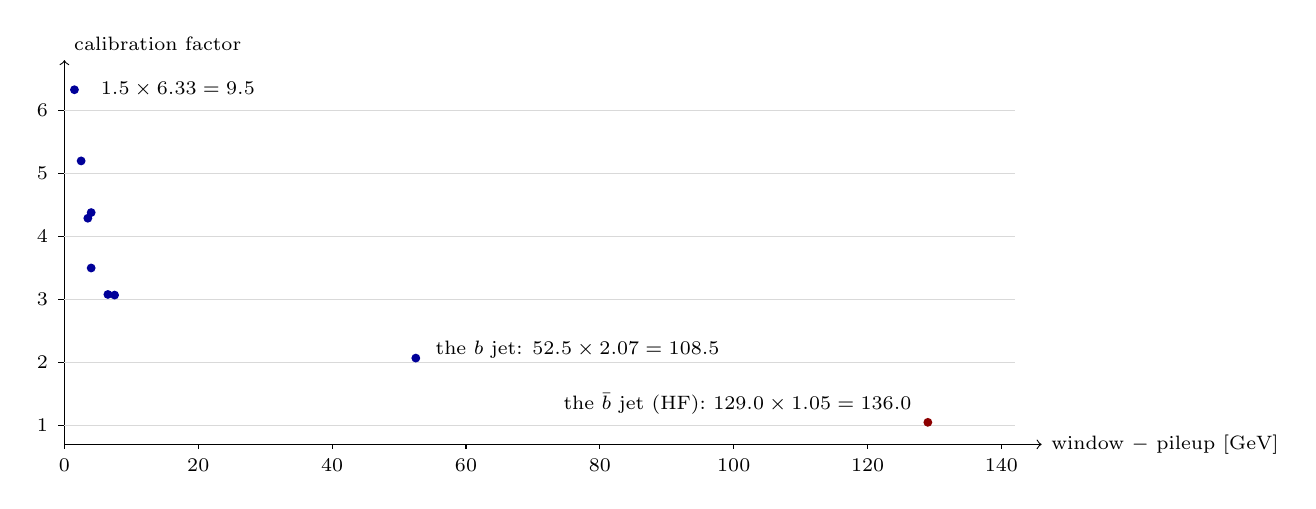
\begin{tikzpicture}[x=0.085cm, y=0.8cm, font=\scriptsize]
\draw[->] (0,0.7) -- (146,0.7) node[right] {window $-$ pileup [GeV]};
\draw[->] (0,0.7) -- (0,6.8) node[above right] {calibration factor};
\foreach \x in {0,20,...,140} \draw (\x,0.7) -- (\x,0.62) node[below] {\x};
\foreach \y in {1,2,3,4,5,6} { \draw (0,\y) -- (-1,\y) node[left] {\y}; \draw[black!15] (0,\y) -- (142,\y); }
\foreach \x/\y in {52.5/2.07, 7.5/3.07, 6.5/3.08, 4/4.38, 3.5/4.29, 4/3.50, 2.5/5.20, 1.5/6.33} \fill[blue!60!black] (\x,\y) circle (1.6pt);
\fill[red!55!black] (129,1.05) circle (1.6pt);
\node[anchor=west] at (54,2.2) {the $b$ jet: $52.5\times2.07=108.5$};
\node[anchor=east] at (128,1.35) {the $\bar b$ jet (HF): $129.0\times1.05=136.0$};
\node[anchor=west] at (4,6.33) {$1.5\times6.33=9.5$};
\end{tikzpicture}
\caption{Step 3, the calibration of the nine jets (table~\ref{tab:12_alljets}): the factor by which Layer-2
multiplies what is left of the window after the pileup subtraction. Blue: barrel and endcap; red: HF. The lookup
table is steep at low energy: a window with $1.5\GeV$ left becomes a jet of $9.5\GeV$.}
\label{fig:12_calib}
\end{figure}


The sums tell the same story in one number each. HTT counts only jets above $30\GeV$ within $\abseta<2.5$, so it
is the $b$ jet alone, $108.5\GeV$: the jet in the HF does not enter it. ETT, the sum of the towers of
barrel and endcap, is $1086\GeV$. The missing transverse energy is real in this event, but small: the neutrino,
$37.5\GeV$ at $\phi=-2.10$ (\code{genMetTrue} of chapter~\ref{ch:06_Decay}). The trigger finds
$\mathrm{ETMHF}=79.0\GeV$ at $\phi=-2.32$, near the neutrino but twice too large: the sum is made of uncalibrated
towers, in which the $b$ jet weighs $74.5\GeV$ and the $\bar b$ jet opposite to it $189\GeV$, and of all the
pileup towers. $\mathrm{HTMHF}$, the same made of the calibrated jets above $30\GeV$, is $34.5\GeV$: the two
signal jets, $136.0$ and $108.5\GeV$ almost back to back. (In 2024 the ring-28 jets entered it and made it $170\GeV$.)

\FloatBarrier
\section{Step 4: muon trigger primitives and track finders}

\textbf{What the step does.} The muon chambers are outside the calorimeters and the return yoke, so that whatever
leaves a line of hits in several stations is, with luck, a muon. Each chamber makes a local track segment, a
\emph{stub}, every 25\,ns. A DT chamber fits the drift times of its layers to a segment with a position and a
bending angle in $\phi$ (\code{simDtTriggerPrimitiveDigis}). A CSC finds a pattern of wire-group hits in its six
layers (the anode pattern, ALCT, which gives $\eta$ and the bunch crossing) and a pattern of half-strips (the
cathode pattern, CLCT, which gives $\phi$ and the bend) and correlates them into one stub, the LCT
(\code{simCscTriggerPrimitiveDigis}); in Run~3 the GEM pads in front of ME1/1 can confirm it. The RPCs send their
hits as they are. Unlike the calorimeter primitives, these are made here, in the L1 job, from the muon digis that
chapter~\ref{ch:11_DIGI} stored. The stubs go to three track finders that divide the detector in $\eta$
(table~\ref{tab:12_tf}). Each is divided in $\phi$ into processors (12 wedges of $30^\circ$ in the barrel, 6
sectors of $60^\circ$ per side elsewhere, 36 processors in all) that link stubs of different stations into a track
and assign it a \pt{} from the bending between stations: the EMTF with a boosted decision tree stored as a lookup
table of $2^{30}$ addresses (\code{PtAssignmentEngine2017}, forest \code{L1TMuonEndCapForest\_v9\_Run3\_2023\_mc}). Each
processor sends up to three candidates, with a quality that says how many stations took part.

\begin{table}[!htb]
\centering\small
\caption{Step 4: the three muon track finders as configured in the L1 job (\code{settings\_12\_L1T.txt}).}
\label{tab:12_tf}
\begin{tabular}{@{}l>{\raggedright\arraybackslash}p{4.1cm}>{\raggedright\arraybackslash}p{4.1cm}>{\raggedright\arraybackslash}p{4.1cm}@{}}
\toprule
 & BMTF (barrel) & OMTF (overlap) & EMTF (endcap) \\
\midrule
region & $\abseta<0.83$ & $0.83<\abseta<1.24$ & $1.24<\abseta<2.4$ \\
stubs & DT segments, with RPC hits merged in by the TwinMux & DT segments, CSC stubs, RPC hits & CSC stubs, RPC hits \\
processors & 12 wedges of $30^\circ$ & 6 sectors of $60^\circ$ per side & 6 sectors of $60^\circ$ per side \\
method & Kalman filter, from the outer station inwards & comparison with stored patterns (the 2024 set, \code{t17}, \code{v3}) & patterns, then \pt{} from a decision-tree table \\
bunch crossings & $-2$ to $+2$ & 0 & $-3$ to $+3$, stubs within 2 \\
module & \code{simKBmtfDigis} & \code{simOmtfDigis} & \code{simEmtfDigis} \\
\bottomrule
\end{tabular}
\end{table}

\textbf{The numbers of the event.} The two $b$ jets give the muon system nothing: the generator event of
chapter~\ref{ch:06_Decay} has no muon above $1\GeV$, and chapter~\ref{ch:10_SIM} found no hit of the signal in any
muon chamber. The event has a muon trigger story all the same (figure~\ref{fig:12_muon}). The 2016 muon digis of
chapter~\ref{ch:11_DIGI} give 11 ALCTs and 8 CLCTs in the CSCs, correlated into 8 LCTs, and 11 GEM pads in 7
clusters; no DT segment. The EMTF receives 12 stubs, 8 CSC and 4 RPC, of which 8 are in bunch crossing 0 (and four
of them a second time: a chamber at the edge of a sector is also given to the neighbouring sector). Four of the
CSC stubs line up:

\begin{center}\small
\begin{tabular}{lcccccc}
\toprule
station & chamber & sector & $\eta$ & $\phi$ & $z$ [cm] & $r$ [cm] \\
\midrule
ME1/1 & 20 & 3 & $-2.084$ & $-2.966$ & $-586$ & 148 \\
ME2/1 & 10 & 3 & $-2.073$ & $-2.875$ & $-815$ & 208 \\
ME3/1 & 11 & 4 & $-2.069$ & $-2.859$ & $-924$ & 237 \\
ME4/1 & 11 & 4 & $-2.067$ & $-2.859$ & $-1014$ & 261 \\
\bottomrule
\end{tabular}
\end{center}

\noindent the same $\eta$ in four stations and a $\phi$ that bends by $0.11$ between the first and the last: a
soft negative particle that crossed the whole endcap. The line happens to cross the boundary between sectors 3
and 4 at $\phi=-165^\circ$, and both sectors find it. Sector 3 owns the first two stubs and builds a two-station
track (``mode 12'': ME1 + ME2) with $\pt=2.0\GeV$ and quality 7; sector 4 owns the last two, receives the first
two as neighbour stubs and builds a four-station track (``mode 15'') with $\pt=3.0\GeV$ and quality 15, the
highest. Two candidates leave the EMTF for one particle. (The ``mode'' is a 4-bit word, one bit per
station, ME1 the highest: 15 is all four stations, 12 the first two. The quality sent to the $\mu$GMT follows from
it, and the algorithms of step~6 ask for a minimum quality: 12 or more for a single-muon algorithm, 8 for a
double-muon one, 4 for the ``open'' ones.)

\begin{plainwords}[Who is this muon]
The file still has the simulated truth of every collision (\code{mix:MergedTrackTruth}, $45\,282$
\code{TrackingParticle}s), and \path{truth_12_L1T.txt} lists what points to the trigger muon: a real $\mu^-$ of
$\pt=2.78\GeV$ at $\eta=-2.08$, from the 21st in-time pileup collision, with 6 tracker hits and 29 hits in the
muon chambers, \emph{produced at $r=58.5\cm$, $z=-214\cm$}, in the middle of the tracker: a decay in flight. The
decay point lies exactly on the line of flight of a $K^-$ of $3.27\GeV$ of the same collision ($\eta=-2.04$, 19
tracker hits), its mother. Not a muon of the hard process, not even a prompt muon: a kaon of the pileup that
happened to decay before the calorimeter. The trigger measured $3.0\GeV$ for $2.78\GeV$.
\end{plainwords}

\begin{figure}[!htb]
\centering
\includegraphics[width=0.8\textwidth]{12_L1T/out/l1t_12_L1T_muon_etaphi_run1_event1.png}\\[4pt]
\includegraphics[width=0.8\textwidth]{12_L1T/out/l1t_12_L1T_muon_rz_run1_event1.png}
\caption{Steps 4 and 5, the muon trigger of the event, in $\eta$--$\phi$ (top) and in $r$--$z$ (bottom)
(\code{l1t\_12\_L1T\_muon\_etaphi/rz\_run1\_event1.png}). Triangles: CSC stubs; dots: RPC stubs (full: bunch crossing 0,
open: another one); red circles: the two EMTF candidates; star and black line: the one muon the $\mu$GMT keeps,
$3.0\GeV$ at $\eta=-2.09$, through the four CSC stations. The dashed lines are the limits of the three track
finders, $\abseta=0.83$, 1.24 and 2.4. The signal jets (magenta) have nothing to do with it. The right panels list
the stubs, the candidates and the muon.}
\label{fig:12_muon}
\end{figure}

\section{Step 5: the global muon trigger}

\textbf{What the step does.} The $\mu$GMT (\code{L1TMuonProducer}) receives up to 108 candidates per bunch
crossing, three from each of the 36 processors, and must hand eight muons to the global trigger. It does three
things. It converts the coordinates, which each processor gives relative to its own sector, to global ones, and
extrapolates each muon from the second muon station back to the vertex through the magnetic field with a lookup
table, because the global trigger wants to compute invariant masses and angles to jets with directions at the
vertex. It removes the \emph{ghosts}: a muon at the border of two sectors, of two wedges, or of two track finders
is found twice, and of two candidates that are close in the coordinates (\code{emtfCancelMode = coordinate}) or
share stubs (\code{bmtfCancelMode = kftracks}) only the one of higher quality is kept. And it sorts what is left
by a rank made of \pt{} and quality and keeps the first eight. It also sums the calorimeter towers around each
muon for an isolation bit (\code{simGmtCaloSumDigis}).

\textbf{The numbers of the event.} The two candidates of step~4 arrive from EMTF processors 2 and 3 of the
negative side with identical coordinates, $(\eta,\phi)=(-2.088,-2.880)$. The $\mu$GMT recognises a ghost,
discards the quality-7 candidate and sends \emph{one} muon: $\pt=3.0\GeV$, charge $-1$, quality 15, at the
vertex $(\eta,\phi)=(-2.066,3.098)$. The extrapolation moved it by $0.31$ in $\phi$, across the $\pm\pi$ line: a
$3\GeV$ track curls that much between the collision point and the second station. Table~\ref{tab:12_gmt} shows the
integers behind it: a transverse momentum in steps of $0.5\GeV$, $\pt=(\mathrm{hwPt}-1)\times0.5\GeV$; a
pseudorapidity in steps of $0.010875$; and an azimuth in units of $2\pi/576$ counted \emph{from the edge of the
processor's own sector}, a sector being 96 units wide. The same muon is at 96, the far edge, for processor 2 and
at 0, the near edge, for processor 3: the two numbers are the same place.

\begin{table}[!htb]
\centering\small
\caption{Step 5: the two EMTF candidates and the muon the $\mu$GMT makes of them (\code{l1t\_12\_L1T.log}, lines
\code{TFCand} and \code{uGMT muon}).}
\label{tab:12_gmt}
\begin{tabular}{@{}l ccc ccc c@{}}
\toprule
 & hwPt & hwEta & hwPhi & \pt{} [GeV] & $\eta$ & $\phi$ & quality \\
\midrule
EMTF, processor 2 (sector 3) & 5 & $-192$ & 96 & 2.0 & $-2.088$ & $-2.880$ & 7 \\
EMTF, processor 3 (sector 4) & 7 & $-192$ & 0 & 3.0 & $-2.088$ & $-2.880$ & 15 \\
\midrule
$\mu$GMT muon, at the second station & & & & 3.0 & $-2.088$ & $-2.880$ & 15 \\
$\mu$GMT muon, at the vertex & & & & & $-2.066$ & $3.098$ & \\
\bottomrule
\end{tabular}
\end{table}

Without the ghost removal the event would have two muons at the same place and would fire every dimuon algorithm
with a low threshold; the menu has 180 algorithms with a muon in them, so this small step protects the rate of
more than a third of the menu.

\FloatBarrier
\section{Step 6: the global trigger}

\textbf{What the step does.} The $\mu$GT (\code{L1TGlobalProducer}) is where the event stops being data and
becomes a decision. Its input is short: at most 12 jets, 12 e/$\gamma$, 12 $\tau$, 8 muons, each a transverse
energy, an $\eta$, a $\phi$ and a few quality bits, plus the energy sums and a few external signals (the beam
pick-ups that say that two filled bunches are crossing). Its program is the \emph{menu}, a list of up to 512
\emph{algorithms}; ours is \code{L1Menu\_Collisions2025\_v1\_0\_0} (the payload \code{L1Menu\_Collisions2025\_v1\_0\_0\_xml}
of \code{L1TUtmTriggerMenuRcd}), with 465 algorithms built from 481 \emph{conditions}. A condition is a
requirement on objects, for example \code{JET90}: ``a jet with $E_{\mathrm T}\geq90\GeV$''; or
\code{JET35[JET-ETA\_2p52]}: the same above $35\GeV$ with $\abseta<2.523$; or \code{mass\_inv\{JET35,JET35\}[MASS\_MIN\_800]}:
two jets above $35\GeV$ with an invariant mass above $800\GeV$. An algorithm is a logical expression of
conditions (AND, OR, NOT) with a name, \code{L1\_SingleJet90}. The firmware evaluates all 465 at once, in a few
bunch crossings. Each algorithm then has a \emph{prescale} $N$ (only one in $N$ of its positive decisions counts;
the low-threshold algorithms need it to fit in the rate) and a mask, and the logical OR of what survives is the
\emph{FinalOR}: 1 means that the event is read out.

Of the 465 algorithms of this menu, 180 involve a muon, 112 an e/$\gamma$, 30 a $\tau$ and 119 only jets and sums
(the 2024 menu had 408: 180, 89, 27 and 93). Fifteen are of a new kind, introduced in 2024: eight
\code{L1\_CICADA\_*} and seven \code{L1\_AXO\_*} cut on an \emph{anomaly score}
computed by a small neural network (for CICADA an autoencoder on the $18\times14$ calorimeter regions of Layer-1,
\code{simCaloStage2Layer1Summary}), which is large for an event that does not look like the bulk of the collisions.

\begin{plainwords}[The simulation runs without prescales]
The emulator is configured with \code{AlgorithmTriggersUnprescaled = True} and \code{AlgorithmTriggersUnmasked =
True} (\path{L1Trigger/L1TGlobal/python/simGtStage2Digis_cfi.py}), and the prescale payload of the global tag is
called \code{L1TGlobalPrescalesVetos\_passThrough\_mc}. Every algorithm has prescale 1, so in the simulation ``fired''
and ``kept'' are the same thing, and \code{L1\_ZeroBias}, which only asks that two bunches cross, fires on every
event: the FinalOR of a simulated event is always 1. In data the prescale column of the run decides, and
\code{L1\_ZeroBias} keeps one crossing in many thousands. The question to ask of a simulated event is therefore not
``is the FinalOR 1'' but ``which algorithms fired'', and which of them the analysis one has in mind can use.
\end{plainwords}

\textbf{The numbers of the event.} 63 of the 465 algorithms fire. Eight of them do not look at any object and
would fire on any simulated crossing: \code{L1\_ZeroBias}, its copy, \code{L1\_AlwaysTrue}, the three beam pick-up
algorithms and the two minimum-bias algorithms that ask for one HF tower on each side. Table~\ref{tab:12_algos}
lists the other 55 with the objects that satisfy them, which the emulator records for every condition (the object
map, printed in the log), and figure~\ref{fig:12_ladders} shows where the event stands on the thresholds of the
menu.

\begin{table}[!htb]
\centering\footnotesize
\caption{Step 6: the 55 algorithms of \code{L1Menu\_Collisions2025\_v1\_0\_0} that fire on an object of the event, with
what satisfies them and the margin to the threshold (\code{ledger\_12\_L1T.txt}, section 6). 22 are satisfied by
the two signal jets alone; the other 33 need an object that has no generator jet or signal particle behind it.}
\label{tab:12_algos}
\begin{tabular}{@{}>{\raggedright\arraybackslash\ttfamily}p{5.9cm}c>{\raggedright\arraybackslash}p{8.2cm}@{}}
\toprule
\normalfont algorithm (\code{L1\_...}) & \normalfont how many & what satisfies it \\
\midrule
SingleJet35, 60, 90, 120 & 4 & the $\bar b$ jet, $136.0\GeV$ (the $b$ jet, $108.5\GeV$, also satisfies the first three): 120 passed by $16\GeV$, 180 failed by $44\GeV$ \\
SingleJet35er2p5, SingleJet60er1p3to2p5 & 2 & the $b$ jet ($\abseta<2.52$; $1.3<\abseta<2.52$); \code{120er2p5} failed by $11.5\GeV$ \\
SingleJet35, 60, 90, 120\_FWD2p5; SingleJet35, 120\_FWD3p0 & 6 & the $\bar b$ jet ($\abseta>2.48$; $\abseta>3.0$) \\
SingleJet8erHE, 10erHE, 12erHE & 3 & the $b$ jet ($1.39<\abseta<2.96$), and a pileup jet of $17.5\GeV$ \\
SingleJet8, 8er2p13; SingleJet8, 12, 16, 20, 24\_BptxAND & 7 & the two signal jets; low-threshold algorithms new in the 2025 menu, some with the beam pick-up condition \\
\midrule
SingleMuCosmics, SingleMuOpen, each also \_EMTF; SingleMu0\_DQ, SingleMu0\_EMTF, SingleMu3 & 7 & the muon of the kaon decay, $3.0\GeV$, quality 15: \code{SingleMu3} passed by $0\GeV$, \code{SingleMu5} failed by 2 \\
Mu3\_Jet30er2p5 & 1 & that muon and the $b$ jet \\
SingleJet8er1p3; SingleJet8, 12, 16, 20er1p3\_BptxAND & 5 & the pileup jets of $23.0$ and $20.0\GeV$ in the barrel ($\abseta<1.3$) \\
SingleEG5, 7, 5er1p52, 7er1p52, 5\_BptxAND, 7\_BptxAND; DoubleEG2, 2er2p13; DoubleEG2, 3, 4\_BptxAND and their er2p13 & 14 & e/$\gamma$ candidates of $7.5\GeV$ at $\eta=-0.30$ and $7.0\GeV$ at $\eta=-0.70$, in the pileup; \code{SingleEG8er2p5} failed by $0.5\GeV$ \\
ETMHF70, ETMHF70\_HTT60er & 2 & $\mathrm{ETMHF}=79.0\GeV$ (the neutrino has $37.5\GeV$): 70 passed by 9.0, 80 failed by $1.0\GeV$ \\
CICADA\_VLoose, Loose, Medium, Tight & 4 & anomaly score 88.3; thresholds 50, 60, 70, 80; \code{VTight} (90) failed by 1.7 \\
\bottomrule
\end{tabular}
\end{table}

The first five lines of the table read like a description of the signal: a jet above $120\GeV$, a jet above
$35\GeV$ within $\abseta<2.5$, a jet above $120\GeV$ beyond $\abseta=3$, a jet in the endcap. These 22 algorithms
are satisfied by the two jets of table~\ref{tab:12_jets}. Even so, the highest of them owes its margin to the
pileup: \code{L1\_SingleJet120} fires on the $\bar b$ jet at $136.0\GeV$, a jet whose generator-level \pt{} is
$115.9\GeV$, below the threshold.

The other 33 algorithms need something that the hard collision did not make: seven single-muon algorithms and a
muon+jet one need the kaon decay of step~4; five barrel-jet and fourteen e/$\gamma$ algorithms with low thresholds
need the pileup jets and clusters of the barrel; two missing-energy algorithms need an ETMHF twice the neutrino; and
the four looser CICADA algorithms an anomaly score of 88.3, between the 80 of \code{L1\_CICADA\_Tight} and the 90 of
\code{L1\_CICADA\_VTight}. Nothing that the 2024 version of this chapter found fires any more on a fake: with no jet
in tower ring 28, none of the vector-boson-fusion algorithms (two jets far apart in $\eta$ with a large invariant
mass) and none of the $H_{\mathrm T}$-imbalance algorithms fires, and of the thirteen missing-energy algorithms of 2024
two are left. The anomaly score was 181.7 in 2024, against thresholds of 113 to 131; the model of 2025 (\code{v2p2p0},
from the era) on the 2024 towers gives 126.4, the model of 2024 on the 2025 towers 127.7: each change alone lowers
the score by a third (companion).

\begin{plainwords}[One algorithm, evaluated by hand]
\code{L1\_DoubleJet\_110\_35\_DoubleJet35\_Mass\_Min800} is the expression \code{comb\{JET110,JET35\} AND
mass\_inv\{JET35,JET35\}[MASS\_MIN\_800]}: two conditions. The first asks for a jet of at least $110\GeV$ and another
of at least $35\GeV$: the $\bar b$ jet ($136.0\GeV$) and the $b$ jet ($108.5\GeV$), the only two above $35\GeV$.
The second asks for two jets above $35\GeV$ with
$M^2/2=E_{\mathrm T1}E_{\mathrm T2}(\cosh\Delta\eta-\cos\Delta\phi)\geq800^2/2=320\,000\GeV^2$ (the menu
stores the cut in this form; the firmware takes $\cosh$ and $\cos$ from lookup tables). For the two signal jets,
$\Delta\eta=2.2$ and $\Delta\phi=2.98$: $136.0\times108.5\times5.65=83\,000$, a mass of $408\GeV$: fails, and
there is no other pair. With the 2024 conditions it fired: a ring-28 jet of $56\GeV$ at $\eta=+2.74$, two thirds of
it calibration factor, six units of rapidity from the $\bar b$ jet, made a ``vector-boson-fusion'' pair of
$2.2\TeV$. The transparency of the crystals at the edge of the endcap decided a VBF trigger.
\end{plainwords}

\begin{figure}[!htb]
\centering
\includegraphics[width=0.93\textwidth]{12_L1T/out/l1t_12_L1T_global_ladders_run1_event1.png}
\caption{Step 6, the ``ladders'' of the menu (\code{l1t\_12\_L1T\_global\_ladders\_run1\_event1.png}). One line per family
of single-object algorithms; the ticks are the thresholds of the menu in GeV, green if the algorithm fired, red if
not; the blue triangle is the event. The right panel gives the margins.}
\label{fig:12_ladders}
\end{figure}

\textbf{The record of one decision.} The emulator keeps, for every algorithm, the conditions and the objects that
satisfied them; the analyzer prints it. For the seed of this book and two of its neighbours
(\path{l1t_12_L1T.log}, objects as (E$_{\mathrm T}$, $\eta$, $\phi$)):

\begin{lstlisting}[style=txt]
fired: bit=302 name=L1_SingleJet90 expression="JET90" | SingleJET_i220=1 (2 combinations): Jet[0](136.0,-3.74,1.00) or Jet[1](108.5,-1.52,-1.98)
fired: bit=307 name=L1_SingleJet35er2p5 expression="JET35[JET-ETA_2p52]" | SingleJET_i224=1 (1 combination): Jet[1](108.5,-1.52,-1.98)
fired: bit=19 name=L1_SingleMu3 expression="MU3[MU-QLTY_SNGL]" | SingleMU_i12=1 (1 combination): Mu[0](3.0,-2.09,-2.88)
\end{lstlisting}

\noindent \code{L1\_SingleJet90} is one condition, \code{JET90}, true for two objects, either of which would have
been enough; with the $\eta$ cut only the $b$ jet remains; and the muon algorithm asks, besides $3\GeV$, for the
quality bits 12 to 15 (\code{MU-QLTY\_SNGL}), which the four-station track of step~4 has.

\textbf{What the decision opens.} A Level-1 algorithm is a \emph{seed}: every path of the High Level Trigger of
chapter 13 starts by asking whether one or a few named algorithms fired, and reconstructs nothing if they did not.
Table~\ref{tab:12_seeds} lists the single-jet paths of the 2025 HLT menu of the release
(\path{HLTrigger/Configuration/python/HLT_2025v10_cff.py}) with their seeds and what our event did with them. For the
analysis this book is heading to, jets, the algorithm that matters is \code{L1\_SingleJet90}, the seed of
\code{HLT\_PFJet110} and \code{HLT\_PFJet140}: our event passes it with a margin of $46\GeV$ on the $\bar b$ jet and
of $18.5\GeV$ on the $b$ jet alone. It is the door through which the event enters chapter 13.

\begin{table}[!htb]
\centering\small
\caption{Step 6: the Level-1 seeds of the single-jet HLT paths (\code{L1SeedsLogicalExpression} of the \code{hltL1s*}
modules of \code{HLT\_2025v10\_cff.py}) and their decision for our event (\code{l1t\_12\_L1T.log}, lines \code{algo:}).}
\label{tab:12_seeds}
\begin{tabular}{@{}>{\raggedright\arraybackslash}p{5.4cm}>{\raggedright\arraybackslash}p{3.9cm}>{\raggedright\arraybackslash}p{6.4cm}@{}}
\toprule
Level-1 seed & our event & HLT paths it opens \\
\midrule
\code{L1\_ZeroBias} & fired (always, in the simulation) & \code{HLT\_PFJet40}, \code{60}, \code{80}; \code{HLT\_PFJetFwd40}, \code{60} \\
\code{L1\_SingleJet90} & fired, by $46.0\GeV$ & \code{HLT\_PFJet110}, \code{HLT\_PFJet140} \\
\code{L1\_SingleJet120} & fired, by $16.0\GeV$ & \code{HLT\_PFJet200} \\
\code{L1\_SingleJet160er2p5 OR L1\_SingleJet180 OR L1\_SingleJet200} & not fired (180 failed by $44.0\GeV$) & \code{HLT\_PFJet260} to \code{550}; \code{HLT\_PFJetFwd260} to \code{500} \\
\code{L1\_SingleJet60\_FWD2p5} & fired & \code{HLT\_PFJetFwd80} \\
\code{L1\_SingleJet90\_FWD2p5} & fired & \code{HLT\_PFJetFwd140} \\
\code{L1\_SingleJet120\_FWD2p5} & fired & \code{HLT\_PFJetFwd200} \\
\bottomrule
\end{tabular}
\end{table}

\FloatBarrier
\section{Ledger and display}

A checkpoint has a ledger with two parts that never mix. The first is the energy the trigger \emph{sees}, step by
step (table~\ref{tab:12_ledger}, top); nothing of it is added to or taken from the recorded event, whose digis are
those of chapter~\ref{ch:11_DIGI}, untouched. The second is the decision (bottom).

\begin{table}[!htb]
\centering\small
\caption{The ledger of the Level-1 trigger (\code{ledger\_12\_L1T.txt}). Top: the transverse energy seen at each
step, in GeV, and what the step did to it. Middle: the objects handed from step to step. Bottom: the decision.}
\label{tab:12_ledger}
\begin{tabular}{@{}p{8.2cm} r l@{}}
\toprule
\multicolumn{3}{@{}l}{\emph{energy seen (GeV)}} \\
step 1: $\sum E_{\mathrm T}$ of the ECAL primitives & 1047.5 & \\
step 1: $\sum E_{\mathrm T}$ of the HCAL primitives (with HF) & 1745.5 & \\
step 2: $\sum E_{\mathrm T}$ of the Layer-1 towers & 2181.0 & $-612.0$ removed by Layer-1 \\
step 3: ETT (towers, $|i\eta|\leq28$) & 1086.0 & \\
step 3: sum of the $9\times9$ windows of the 9 jets & 440.5 & \\
step 3: sum of the jet $E_{\mathrm T}$ (subtracted, calibrated) & 356.5 & $-229.5$ pileup estimates \\
step 3: HTT (jets $>30\GeV$, $\abseta<2.5$) & 108.5 & \\
step 3: ETM / ETMHF & 60.5 / 79.0 & the neutrino: 37.5 \\
step 3: HTM / HTMHF & 108.0 / 34.5 & \\
\midrule
\multicolumn{3}{@{}l}{\emph{objects}} \\
step 1: primitives with $E_{\mathrm T}>0$ & 2479 & of 8856 \\
step 2: towers with $E_{\mathrm T}>0$ & 2561 & of 5760 \\
step 3: jets / e/$\gamma$ / $\tau$ sent to the $\mu$GT & 9 / 12 / 12 & of at most 12 each \\
\quad L1 jet of the $b$ jet & 108.5 & generator 117.8 (79.8 visible) \\
\quad L1 jet of the $\bar b$ jet & 136.0 & generator jet 115.9 \\
step 4: CSC stubs (LCT) / stubs given to the EMTF & 8 / 12 & \\
step 4: candidates of BMTF / OMTF / EMTF & 0 / 0 / 2 & \\
step 5: muons sent to the $\mu$GT & 1 & 3.0 GeV, a pileup kaon decay \\
\midrule
\multicolumn{3}{@{}l}{\emph{decision}} \\
step 6: algorithms fired & 63 & of 465 \\
\quad that look at an object & 55 & \\
\quad satisfied by the two signal jets alone & 22 & \\
\quad highest single-jet threshold passed & 120 & by 16.0 GeV \\
\quad \code{L1\_SingleJet90}, the seed of \code{HLT\_PFJet110} & fired & by 46.0 GeV \\
\quad CICADA anomaly score & 88.3 & \code{Tight} (80) passed, \code{VTight} (90) not \\
FinalOR & 1 & \\
\bottomrule
\end{tabular}
\end{table}

Read downwards, the table is the price of speed and of pileup together. The collision put two jets of $80$ and
$116\GeV$ of visible particles in the detector. At step~1 the trigger sees $2793\GeV$ of transverse energy,
four fifths of it pileup and noise. Layer-1 removes $612\GeV$ with its thresholds, and the $\phi$-ring subtraction
of Layer-2 another $229.5\GeV$ from the jet windows; what is left is nine jets and $356.5\GeV$, of which the two
real jets are $244.5\GeV$. The global trigger then says yes 63 times, 22 of them for the two jets the journey has
followed since chapter~\ref{ch:01_ME}. The one algorithm the journey needs is among those 22.

\paragraph{What the year changed.} The same event on the 2024 settings (the first version of this chapter; the
companion compares the two step by step) gave $3411.5\GeV$ of primitives, twelve jets, six of them seeded in tower
ring 28, and 57 of 408 algorithms, among them eight VBF and five $H_{\mathrm T}$-imbalance algorithms fired by those
jets. The 2025 crystals at the edge of the endcap give a quarter of the light, the ring-28 jets are gone, and with
them every algorithm they fired. The two signal jets moved by $+2$ and $-1\GeV$, the muon not at all, and
\code{L1\_SingleJet90} fires as before.

\begin{figure}[!htb]
\centering
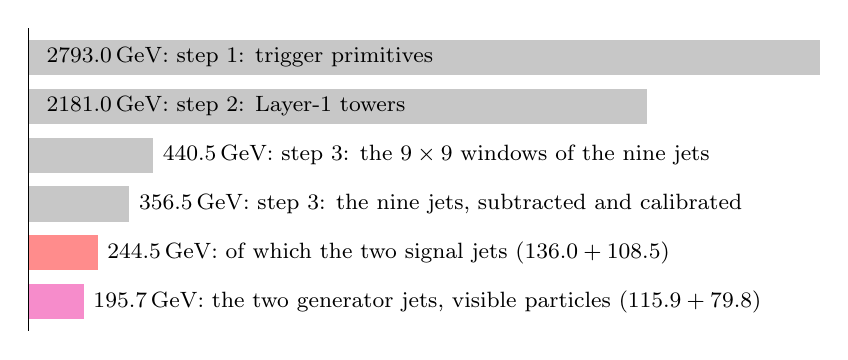
\begin{tikzpicture}[x=0.0036cm, y=0.62cm, font=\footnotesize]
\foreach \y/\v/\c/\t in {5/2793.0/black!22/{step 1: trigger primitives},
                         4/2181.0/black!22/{step 2: Layer-1 towers}}
{ \fill[\c] (0,\y-0.36) rectangle (\v,\y+0.36); \node[anchor=west] at (30,\y) {\v\,GeV: \t}; }
\foreach \y/\v/\c/\t in {3/440.5/black!22/{step 3: the $9\times9$ windows of the nine jets},
                         2/356.5/black!22/{step 3: the nine jets, subtracted and calibrated},
                         1/244.5/red!45/{of which the two signal jets ($136.0+108.5$)},
                         0/195.7/magenta!45/{the two generator jets, visible particles ($115.9+79.8$)}}
{ \fill[\c] (0,\y-0.36) rectangle (\v,\y+0.36); \node[anchor=west] at (\v,\y) {\v\,GeV: \t}; }
\draw (0,-0.6) -- (0,5.6);
\end{tikzpicture}
\caption{The energy part of the ledger as a picture: the transverse energy the trigger holds at each step
(table~\ref{tab:12_ledger}), down to the two jets it is looking for.}
\label{fig:12_funnel}
\end{figure}

Figure~\ref{fig:12_objects} is the display of the event at the end of the chapter: all that is left of it for the
global trigger. Compare it with figure~\ref{fig:11_mixed}, the $544\,407$ digis of the same event: the two magenta
circles are again the only thing the two pictures share, and now each has a red square in it.

\begin{figure}[!htb]
\centering
\includegraphics[width=0.93\textwidth]{12_L1T/out/l1t_12_L1T_global_objects_run1_event1.png}
\caption{The event as the global trigger receives it: 9 jets, 12 e/$\gamma$, 12 $\tau$, 1 muon and the sums
(\code{l1t\_12\_L1T\_global\_objects\_run1\_event1.png}). Red squares: jets with their $E_{\mathrm T}$ in GeV; blue
triangles: $\tau$ candidates; green dots: e/$\gamma$ candidates; star: the muon; the ticks on the left edge: the
direction of the missing transverse energy with HF (orange) and of the missing $H_{\mathrm T}$ (violet). Magenta
circles: the two generator jets.}
\label{fig:12_objects}
\end{figure}

\FloatBarrier
\section{Open problems for Phase-2}

The Phase-2 Level-1 trigger is a different machine: it has the tracker (tracks above $2\GeV$ at 40\,MHz), a
particle-flow reconstruction and PUPPI in firmware (the \emph{correlator}), the HGCAL in the endcaps, a latency of
$12.5\,\mu$s and an output rate of 750\,kHz. What follows is what the release, CMSSW\_15\_0\_5 with the era
\code{Phase2C17I13M9}, says about its state.

\textbf{The Run-3 trigger of this chapter still runs in Phase-2, on Run-3 primitives.} In
\path{L1Trigger/Configuration/python/SimL1Emulator_cff.py} the Phase-2 emulation is built as
\code{\_phase2\_siml1emulator = SimL1EmulatorTask.copy()} (line 62) and substituted under \code{phase2\_trigger} (line
279): a copy of the task of this chapter with modules added. Layer-1, Layer-2, the three track finders, the
$\mu$GMT and the $\mu$GT of Run~3 are all still executed on the Phase-2 detector; no modifier removes them
(\path{L1Trigger/L1TCalorimeter/python/simDigis_cff.py}, \path{L1Trigger/L1TMuon/python/simDigis_cff.py}, where
\code{phase2\_trigger} lists \code{simBmtfDigis}, \code{simEmtfDigis}, \code{simGmtStage2Digis} explicitly). The header
of the file says of the forward calorimeter: ``At the moment, there is no emulator available for upgrade HF Trigger
Primitives, so these missing (required!) inputs are presently ignored by downstream modules.'' The HCAL
trigger-primitive emulator of chapter~\ref{ch:11_DIGI} has no Phase-2 modifier at all
(\path{SimCalorimetry/HcalTrigPrimProducers/python/hcaltpdigi_cfi.py}: the last modifiers are \code{run3\_HB} and
\code{run3\_common}), and the Phase-2 calorimeter-trigger modules read \code{simHcalTriggerPrimitiveDigis}, the
collection of step~1 of this chapter. The Phase-2 ECAL barrel primitive (one per crystal, the reason for the new
barrel electronics) exists as \code{simEcalEBTriggerPrimitivePhase2Digis} but is switched on only by
\code{phase2\_ecalTP\_devel} (\path{SimCalorimetry/Configuration/python/ecalDigiSequence_cff.py}), a modifier that no era
includes; the era uses \code{simEcalEBTriggerPrimitiveDigis}, made from the Run-3 digitisation that
chapter~\ref{ch:11_DIGI} found in the same state.

\textbf{The pileup subtraction of the Phase-2 calorimeter towers was fitted in 2019.} The module that plays the
role of our Layer-1 (\path{l1tTowerCalibrationProducer_cfi.py} in \path{L1Trigger/L1CaloTrigger/python/}) opens with
``Choosen settings 6 March 2019, 10\_3\_X MTD samples''; its pileup estimate counts the towers hit, converts the count
to a number of vertices and the number of vertices to an energy per tower with ``Parameters derived on 6 March
2019 on 10\_3\_X MTD samples''. The 2024 calorimeter-jet emulator (\path{l1tPhase2CaloJetEmulator_cfi.py}) carries the
same numbers without the comment, under jet calibrations ``derived 26 June 2024 on 14\_0\_0\_pre3 131X QCD sample''.
This chapter showed for PU 60 what such an estimate is worth when the detector is not uniform (a jet's own energy
in its rings; tower ring 28, whose response changed by a factor of three between two global tags): scaled linearly
to PU 200 the towers of step~2 would hold some $7\TeV$, and the estimate that decides how much of it is a jet is a
fit on 2019 samples.

\textbf{A sum that is always zero.} Line 115 of \path{SimL1Emulator_cff.py} configures the Phase-2 calorimeter
$H_{\mathrm T}$ with \code{BXVCaloJetsInputTag = ("L1CaloJet", "CaloJets")}. No module has the label \code{L1CaloJet}:
the producer of line 108 is \code{l1tCaloJet}, and the collection it writes is called
\code{L1CaloJetCollectionBXV} (\path{L1Trigger/L1CaloTrigger/plugins/L1CaloJetProducer.cc}, line 341). In
the producer of the sum, \path{L1CaloJetHTTProducer.cc} of the same directory, the value is set to 0 and filled
only \code{if (bxvCaloJetsHandle.isValid())}:
the product is written, with the value 0, for every event. Nothing fails because nothing reads it: the Phase-2
global trigger takes no calorimeter jet at all (below).

\textbf{The Phase-2 jets are particle-flow jets, with corrections of March 2022 and cuts ``to be tuned''.} The jets
the Phase-2 global trigger receives are \code{l1tSC4PFL1PuppiCorrectedEmulator}, a seeded cone of radius 0.4 on
PUPPI candidates (\path{L1Trigger/Phase2L1GT/python/l1tGTProducer_cff.py}); the calorimeter jets above are not an
input. Their energy correction is \path{L1Trigger/Phase2L1ParticleFlow/data/jecs/jecs_20220308.root}
(\path{l1pfJetMet_cff.py}), and the cone of radius 0.8 uses the same file with the same directory,
\code{L1PuppiSC4EmuJets}: the wide jets are corrected as narrow ones. The hadron calibrations of the candidates
under them are tagged with the 11\_0\_X release (\code{hadcorr\_barrel\_110X.root}, \code{hfcorr\_110X.root},
\code{hadcorr\_HGCal3D\_TC\_110X.root}). The PUPPI parameters of \path{l1ctLayer1_cff.py} are annotated ``ballpark pT
from PU'' and ``ballpark alpha from PU''; in the HF, where our $\bar b$ jet is and where there are no tracks to
tell the pileup, a candidate needs $10\GeV$ (\code{ptCut}), the sort keeps ten per region (``to be tuned'') and
four buffer sizes are ``to be defined''. The vertex against which all of this is done is the single best one of a
histogram of track $z$ (\code{Algorithm = fastHisto}, \code{FH\_NVtx = 1},
\path{L1Trigger/VertexFinder/python/l1tVertexProducer_cfi.py}), with a comment that the track-\pt{} saturation
differs between the Technical Design Report and the firmware.

\textbf{The HGCAL trigger primitives are calibrated for an older HGCAL.} The era includes the modifiers
\code{phase2\_hgcalV10}, \code{V11} and \code{V16} together, and the trigger takes its settings from the first two:
\path{L1Trigger/L1THGCal/python/l1tHGCalBackEndLayer1Producer_cfi.py} switches the layer calibration off with ``we
still don't have layer calibrations for $>=$V9 geometry'', the trigger geometry class is
\code{HGCalTriggerGeometryV9Imp3}, and the e/$\gamma$ identification in use (\code{v10\_3151}) was ``trained using
TPG software version 3.15.1''.

\textbf{The Phase-2 menu is ``the first prototype menu''.} The Phase-2 global trigger is a separate
\code{cmsDriver} step (\code{L1P2GT}) whose default menu is \code{step1\_2024}
(\path{Configuration/Applications/python/ConfigBuilder.py}, line 1597;
\path{L1Trigger/Configuration/python/Phase2GTMenus/step1_2024.py} begins with the comment quoted). It has 40
algorithms against the 465 of this chapter. The jet ones are \code{pSinglePuppiJet230},
\code{pDoublePuppiJet112\_112}, \code{pPuppiHT450}, \code{pPuppiMHT140}, \code{pPuppiMET200} and a four-jet one; the
numbers are offline thresholds, translated to trigger thresholds with linear ``scalings'' (for jets in the barrel
an offset of $17.33\GeV$ and a slope of 1.28) that ``correspond to version v44 derived with the Annual Review 2024
config in the 14\_2\_x release'', one release series behind this one. There is no single-jet algorithm below
$230\GeV$, no prescaled ladder like \code{SingleJet35/60/90/120}, and the file named for $b$ tagging holds only
multi-muon seeds: an event like ours, two $b$ jets of $115\GeV$, has no hadronic way into the Phase-2 menu as it
stands, and the jet triggers on which jet calibration relies are not written yet.

\textbf{The Run-3 emulation itself is not uniform in time.} The simulated 2025 trigger of this chapter is
assembled from payloads of different years: the calorimeter parameters \code{2024\_v0\_1} (the release has
\code{v0\_3} and two 2025 versions in python), with, in the python of that version, jet compression tables
\code{2017v1} and the jet calibration \code{lut\_calib\_2023v0\_ECALZS\_PhiRing}; seven of the nineteen ECAL
trigger-primitive payloads \code{2018\_mc}; the HCAL ones \code{2019} and \code{2024}; the barrel muon parameters
\code{Stage2v1\_2018\_mc}; the menu of 2025 on the scales \code{scales\_2024\_05\_15}; and in the EMTF the era
\code{Run3\_2021} selects \code{PtAssignmentEngine2017} with the comment ``TODO - implement ver 2021''
(\path{L1Trigger/L1TMuonEndCap/src/EMTFSetup.cc}). The CSC shower thresholds of 2025 that \code{run3\_CSC\_2025} sets
are never used: the modifier writes \code{showerParams}, the producer reads \code{showerParam}
(\path{L1Trigger/CSCTriggerPrimitives/src/CSCBaseboard.cc}). The prescales are absent. Whoever compares a simulated
trigger efficiency with data should know which of the six steps were simulated as of 2025.
